
In this chapter, we investigate various subset mapping and synchronization problems on automata,
which we introduce in \cref{compl:sec:problems}.
\Cref{compl:sec:reductions} explores
reductions and relations between them.
In \cref{compl:sec:subclasses} we investigate the computational
complexity of these problems on general automata
and the subclasses of solvable, commutative, and partially
ordered automata. We give a classification of the (classical) 
complexity landscape and close some gaps from the literature.

\section{The Problems}
\label{compl:sec:problems}

%!TEX root = ./../../springer-mono-format/book.tex
%!TEX root = ./../../thesis-trier.tex

Here, we list the automata-theoretical decision problems of interest to us.

Recall that in \cref{prelim:sec:encodings} we discussed how we encode automata as inputs,
and that here, automata have a totally defined transition function.

\IN{\DFAS}
\decisionproblem{\DFAS (\v{C}ern\'y~\cite{Cer64})}
{Automaton $\semiautomat{A}{Q}{\Sigma}{\delta}$.}
{Is $\Syn(\mathcal A) \ne \emptyset$?}

\IN{\DFAST}
\decisionproblem{\DFAST}
{Automaton $\semiautomat{A}{Q}{\Sigma}{\delta}$ with trap state.}
{Is $\Syn(\mathcal A) \ne \emptyset$?}

\IN{\DFASS}
\decisionproblem{\DFASS}
{Automaton $\semiautomat{A}{Q}{\Sigma}{\delta}$ and state $q \in Q$.}
{Does there exist $u \in \Sigma^*$ such that $\applytrans{\delta}{Q}{u} = \{q\}$?}

\IN{\DFASW}
\decisionproblem{\DFASW}
{Automaton $\semiautomat{A}{Q}{\Sigma}{\delta}$ and finite list of words $u_1, \ldots, u_k \in \Sigma^*$.}
{$\exists i \in \{1,\ldots, k\} : |\applytrans{\delta}{Q}{u_i}| = 1$?}

\IN{\DFASWS}
\decisionproblem{\DFASWS (Rystsov~\cite{Rys80}, Eppstein~\cite{Eppstein90})}
{Automaton $\semiautomat{A}{Q}{\Sigma}{\delta}$ and $l \ge 0$.}
{Is $\Syn(\mathcal A) \cap \Sigma^{\le l} \ne \emptyset$?}

\IN{\SFS}
\decisionproblem{\SFS (Rystsov~\cite{Rys83})\footnote{Called \emph{(global) inclusion problem for weakly-initial automata with a single final state} in~\cite{Rys83}.}}
{Automaton $\semiautomat{A}{Q}{\Sigma}{\delta}$ and $S \subseteq Q$.}
{Does there exist $u \in \Sigma^*$ such that $|\applytrans{\delta}{S}{u}| = 1$?}

\IN{\SIS}
\decisionproblem{\SIS (Rystsov~\cite{Rys83})\footnote{Called \emph{(global) inclusion problem for non-initial automata} in~\cite{Rys83}.}}
{Automaton $\semiautomat{A}{Q}{\Sigma}{\delta}$ and $S \subseteq Q$.}
{Does there exist $u \in \Sigma^*$ such that $\applytrans{\delta}{Q}{u} \subseteq S$?}

\IN{\ST}
\decisionproblem{\ST (Rystsov~\cite{Rys83}, Luks and McKenzie~\cite{LuksM88}, Blondin et al.~\cite{BlondinKM16})\footnote{Called \emph{(global) inclusion problem for weakly initial automata} in~\cite{Rys83}.}}
{Automaton $\semiautomat{A}{Q}{\Sigma}{\delta}$ and $S, T \subseteq Q$.}
{Does there exist $u \in \Sigma^*$ such that $\applytrans{\delta}{S}{u} \subseteq T$?}

\IN{\DST}
\decisionproblem{\DST}
{Automaton $\semiautomat{A}{Q}{\Sigma}{\delta}$ and $S, T \subseteq Q$ with $S \cap T = \emptyset$.}
{Does there exist $u \in \Sigma^*$ such that $\applytrans{\delta}{S}{u} \subseteq T$?}

\IN{\DFAINT}
\decisionproblem{\DFAINT (Kozen~\cite{Kozen77})}
{List of automata $\mathcal A_1, \ldots, \mathcal A_k$ as language acceptors.}
{Do we have $\bigcap_{i=1}^k L(\mathcal A_i) \ne \emptyset$?}

\IN{\REACH}
\decisionproblem{\REACH (Rystsov~\cite{Rys83}, Bondar and Volkov~\cite{BondarV16})}
{Automaton $\mathcal A = (Q, \Sigma, \delta)$ and $S \subseteq Q$.}
{Does there exist $u \in \Sigma^*$ such that $\delta(Q, u) = S$?}

\IN{\REACHF}
\decisionproblem{\REACHF (Rystsov~\cite{Rys83})}
{Automaton $\mathcal A = (Q, \Sigma, \delta)$ and $S,T \subseteq Q$.}
{Does there exist $u \in \Sigma^*$ such that $\delta(S, u) = T$?}

\section{Reductions}
\label{compl:sec:reductions}

%!TEX root = ./../../springer-mono-format/book.tex
%!TEX root = ./../../thesis-trier.tex

Here, in \cref{compl:prop:reductions}, we state various $\leACZEROm$-reductions that work for any fixed alphabet. 
Omitting the $\AC^0$-equivalent problems,
the problems and the reductions from \cref{compl:prop:reductions}
are depicted in the form of a Haase diagram in \cref{prelim:classes:fig:reductions}.
\Cref{compl:prop:reductions_trap,compl:prop:reductions_comm,compl:prop:reductions_unary-SWS-SW}
give some further reductions for classes of automata.
\Cref{prelim:compl:prop:unary-binary} shows that in \DFASWS,
it does not matter whether we encode the length parameter in unary or binary
up to $\leACZEROm$-equivalence.

\begin{remark}
The reductions in \cref{compl:prop:reductions,compl:prop:reductions_trap,compl:prop:reductions_comm} 
involving automata do not change the alphabet.
So, they can be used when we investigate problem 
variants where the alphabet is fixed (as in some statements in~\cref{compl:sec:subclasses}).
Furthermore, because they do not require
that the alphabet is held fixed, they can also be used
for complexity upper bounds when the alphabet is part of the input.
\end{remark}

\begin{figure}[ht]
	\centering
\begin{tikzpicture}[node distance = 0.5cm and 1.5cm]
	\node (scp) {\SCP};
	\node (stp) [above = of scp] {\DFAST};
	\node (syc) [above right = of stp] {\DFAS};
	\node (dss) [above left = of stp]  {\DFASS};
	\node (dsf) [above left = of syc, xshift=1.2cm] {\SFS};
	%\node (sws) [above right = of stp] {\DFASWS};
	\node (sis) [above left  = of dss, xshift=1.2cm] {\SIS};
	\node (rea) [above right = of dss, xshift=-1.2cm] {\REACH};
	\node (dst) [above = of sis] {\ST};
	\node (ref) [above = of rea] {\REACHF}; 
	\node (dws) [above right = of syc, xshift=-1.2cm] {\DFASWS};
	
	\draw[-] (scp) -- (stp);
	\draw[-] (stp) -- (dss) -- (sis) -- (dst);
	\draw[-] (dss) -- (rea) -- (ref);
	\draw[-] (stp) -- (syc) -- (dsf);	
	\draw[-] (syc) -- (dws);
\end{tikzpicture}
	\caption[Haase diagram for reductions]{Haase diagram of the reductions from \cref{compl:prop:reductions}; those equivalent to \ST omitted.}
	\label{prelim:classes:fig:reductions}
\end{figure}

\begin{proposition}
	\label{compl:prop:reductions}
	Fix a non-empty alphabet $\Sigma$. 
	Then the following statements hold:
	\begin{enumerate}				
		\item \label{compl:prop:reductions:item:SCP_DFAST} $\SCP \leACZEROm \DFAST$,
		\item \label{compl:prop:reductions:item:DFAST_DFAS} $\DFAST \leACZEROm \DFAS$,
		\item \label{compl:prop:reductions:item:st-ss} $\DFAST \leACZEROm \DFASS$,	
		\item \label{compl:prop:reductions:item:DFAS_DFASWS} $\DFAS \leACZEROm \DFASWS$,
		\item \label{compl:prop:reductions:item:DFAS_SFS} $\DFAS \leACZEROm \SFS$,
		\item \label{compl:prop:reductions:item:DFASS_SIS} $\DFASS \leACZEROm \SIS$ and $\DFASS \leACZEROm \REACH$,		
		\item \label{compl:prop:reductions:item:REACH-REACHF} $\REACH \leACZEROm \REACHF$,		
		\item \label{compl:prop:reductions:item:SIS_ST} $\SIS \le_m^{\AC^0} \ST$,		
		\item \label{compl:prop:reductions:item:DFAINT_DST}	\label{compl:prop:reductions:item:DFAINT_ST} $\DFAINT \eqACZEROm \ST$, 		
		\item \label{compl:prop:reductions:item:DST_ST} $\DST \eqACZEROm \ST$.
	\end{enumerate} 
	Furthermore, besides preserving the alphabet, the reductions used in \crefrange{compl:prop:reductions:item:DFAST_DFAS}{compl:prop:reductions:item:DST_ST}  
	transform a commutative (resp.~partially ordered, solvable, permutation) automaton
	into a commutative (resp.~partially ordered, solvable, permutation) automaton.
\end{proposition}
\begin{proof}  	
	The following reductions given in \crefrange{compl:prop:reductions:item:SCP_DFAST}{compl:prop:reductions:item:DST_ST}
	below can be easily implemented by \LOGSPACE-uniform circuit families
	in $\AC^0$. Further, for each reduction involving automata, the alphabet is not altered and 
	it is readily seen that when it is applied to a commutative (resp.~partially ordered)
	automaton it yields a commutative (resp.~partially ordered) automaton.
		
	\ref{compl:prop:reductions:item:SCP_DFAST}: 
	Let $g \colon [n] \to [n]$ be a input permutation to \SCP. 
	Set~$\semiautomat{A}{[n]}{\Sigma}{\delta}$
	where, for $x \in \Sigma$,
	$\applytrans{\delta}{0}{x} = 0$
	and $\applytrans{\delta}{i}{x} = \applyfunc{i}{g}$
	for $i \in [n] \setminus \{0\}$.
	Then~$\mathcal A$ has $0$ as a unique synchronizing trap state if and only if~$g$ has a single cycle.	
	
	Note that~$\mathcal A$ has the form of a single tail with a trap state at the end
	if it is synchronizing. But this is not the case 
	if~$g$ has multiple cycles, since then
	the automaton also has at least one cycle.
		
	\ref{compl:prop:reductions:item:DFAST_DFAS}: This is obvious.	 
	
	\ref{compl:prop:reductions:item:st-ss}:	
	We assume the $n$-state input $\mathcal A$ to \DFAST is given as a list 
	of transition matrices $(m_{ij}^{(a)})_{i,j \in \{1,\ldots,n\}}$
	for each $a \in \Sigma$,
	and the input to \DFASS  
	is supplied as a list of transition
	matrices and a vector
	with a one indicating the state to which we want to synchronize
	and zero at all other positions.
	The state~$i$ is a trap state if and only if $m_{ii}^{(a)} = 1$
	for all $a \in \Sigma$.
	Let 
	\[
	b_i = \left( \bigwedge_{a \in \Sigma} m_{ii}^{(a)} \right) 
	\land 
	\left(\bigwedge_{j=1}^{i-1} \bigvee_{a \in \Sigma} \neg m_{jj}^{(a)} \right).
	\]
	Each $b_i$ can be computed by a circuit family in $\AC^0$ 
	by directly implementing the defining formula.
	We have $b_i = 1$ if and only if $i$ is a trap state
	and the other states are not trap states. 
	%Hence $(b_1, \ldots, b_n)$
	%contains at most a single one and zero everywhere else.
	For $b_1 = \cdots = b_n = 0$ we feed a fixed non-synchronizing two-state automaton
	with some state to \DFASS. 
	Otherwise, $(b_1, \ldots, b_n)$ contains the entry~``$1$'' precisely once at a position corresponding to a unique trap state.	
	Then, the transition matrices together with $(b_1, \ldots, b_n)$ 
	are an encoding of an input instance for \DFASS
	that is an \rYES-instance if and only if the original automaton
	is synchronizing.	
		
	\ref{compl:prop:reductions:item:DFAS_DFASWS}:  Let $\mathcal A$ be an $n$-state input automaton to \DFAS. 
	A shortest synchronizing word has length at most $(n^3 - n) / 6$, see \cref{tab:reset_length_bounds} in \cref{intro:sec:cerny}. 
	So, $\mathcal A$ has a synchronizing word
	if and only if $(\mathcal A, n^3)$ is a \rYES-instance
	of \DFASWS. 
	The number of states~$n$ can be readily computed from the input~$\mathcal A$
	and~$n^3$ can be easily computed by circuits constructible by deterministic log-space Turing transducers. 
	Thus the input $(\mathcal A, n^3)$ can be computed
	by a \LOGSPACE-uniform family of circuits in~$\AC^0$ (where the encoding of $n^3$
	does not matter by \cref{prelim:compl:prop:unary-binary}).
				
	\ref{compl:prop:reductions:item:DFAS_SFS}: This follows as an automaton $\mathcal A$ is synchronizing 
	if and only if $(\mathcal A, Q)$ is a \rYES-instance of \SFS.	
	
	\ref{compl:prop:reductions:item:DFASS_SIS}: An input instance $(\mathcal A, q)$ of \DFASS can be converted
	readily to an equivalent input $(\mathcal A, \{q\})$
	to \SIS, which is also an equivalent input for \REACH.
	
	\ref{compl:prop:reductions:item:SIS_ST}: The \SIS-instance $(\mathcal A, S)$ 
	is equivalent to the \ST-instance $(\mathcal A, Q, S)$, giving a reduction doable by an \LOGSPACE-uniform circuit family in~$\AC^0$.
			
	\ref{compl:prop:reductions:item:DFAINT_DST}: 
	Let $\semiautomat{A_i}{Q_i}{\Sigma}{\delta_i}$,
	$q_i \in Q_i$, and $F_i\subseteq Q_i$ for $i \in \{1,\ldots,k\}$
	be an input instance for \DFAINT.
	We can assume the state sets $Q_i$ are pairwise disjoint.
	Set $\semiautomat{A}{Q}{\Sigma}{\delta}$ with $Q = Q_1 \cup \cdots \cup Q_k$
	and 
	$
	\applytrans{\delta}{q}{x} = \applytrans{\delta_i}{q}{x} 
	$
	if $q \in Q_i$.
	Then, for $u \in \Sigma^*$, we have $\applytrans{\delta}{\{ q_1, \ldots, q_k\}}{u} \subseteq F_1 \cup \ldots \cup F_k$
	if and only if $\delta_i(q_i, u) \in F_i$ for all $i \in \{1,\ldots,k\}$, giving a reduction
	preserving the alphabet and the mentioned automata types.
	
	Next, let $(\mathcal A, S, T)$ with $\semiautomat{A}{Q}{\Sigma}{\delta}$
	and $S,T \subseteq Q$ be a \ST-instance. 
	Write $S = \{s_1, \ldots, s_m\}$.
	Then, for $i \in \{1,\ldots,m\}$,
	with $\mathcal A_i = \mathcal A$, $q_i = s_i$,
	and $F_i = T$ we obtain an instance of \DFAINT 
	that has a solution if and only if there exists a word
	in $\mathcal A$ mapping $S$ into $T$.        
		
	\ref{compl:prop:reductions:item:DST_ST}: It is sufficient to show
	$\ST \leACZEROm \DST$. Let $\semiautomat{A}{Q}{\Sigma}{\delta}$
	and $S, T \subseteq Q$. We can assume $S \not\subseteq T$.
	Set $\semiautomat{\overline{\mathcal A}}{Q \cup \{0\} \times S}{\Sigma}{\overline{\delta}}$
	where, for $x \in \Sigma$,
	we let $\applytrans{\overline{\delta}}{(0, s)}{x} = \applytrans{\delta}{s}{x}$
	for $s \in S$
	and $\applytrans{\overline{\delta}}{q}{x} = \applytrans{\delta}{q}{x}$
	for $q \in Q$.
	This construction can be implemented by a \LOGSPACE-uniform circuit family in $\AC^0$ as we only add states
	and transitions according to a fixed scheme. 
	For a non-empty word $u \in \Sigma^+$
	we have $\applytrans{\delta}{S}{u} \subseteq T$
	if and only if $\applytrans{\overline{\delta}}{\{0\} \times S}{u} \subseteq T$
	and as $\{0\} \times S$ and $T$ are disjoint this gives a valid reduction.
\end{proof}

\begin{proposition}  \label{compl:prop:reductions_trap}
	For automata whose synchronizing states are trap states
	as, for example, solvable automata,
	we have
	$\DFAS \eqACZEROm \DFASS$ and
	$\DFASS \eqACZEROm \DFAST$.
\end{proposition}
\begin{proof}	
	Let $\semiautomat{A}{Q}{\Sigma}{\delta}$
	be an input automaton and $n = |Q|$.
	We assume $\mathcal A$ is supplied 
	as a list of transition matrices $(m_{ij}^{(a)})_{i,j \in \{1,\ldots,n\}}$, $a \in \Sigma$,
	w.r.t.~to an identification of the states with $\{1,\ldots,n\}$.	
	By \crefitem{compl:prop:reductions}{compl:prop:reductions:item:st-ss}, 
	$\DFAST \leACZEROm \DFASS$.
	Thus, it is sufficient to show
	$
	\DFASS \leACZEROm 
	\DFAS \leACZEROm 
	\DFAST.
	$
	
	\medskip 
	\noindent\underline{$\DFASS \leACZEROm \DFAS$}: Since a trap state must be a unique synchronizing state,
	with the assumption we obtain that a state $q$ in 
	$\mathcal A$
	is synchronizing if and only if $\mathcal A$ is synchronizing
	and~$q$ a trap state.
	So, we first check whether $q$ is a trap
	state by implementing the formula $\bigwedge_{a \in \Sigma} m_{qq}^{(a)}$
	and, if~$q$ is a trap state,
	pass $\mathcal A$ to \DFAS.
	Otherwise, we pass some fixed \rNO-instance
	to \DFAS.
	
	\medskip 
	\noindent\underline{$\DFAS \leACZEROm \DFAST$}:
	Since by assumption a synchronizing state is a trap state,
	$\mathcal A$ is synchronizing if and only if it has a trap 
	state and is synchronizing. Existence of a trap state 
	can be checked by the formula $\bigvee_{i = 1}^n \bigwedge_{a \in \Sigma} m_{ii}^{(a)}$.
	If this check succeeds,	we pass $\mathcal A$ to \DFAST. 
	Otherwise, we pass some fixed \rNO-instance to \DFAST.
\end{proof}

\begin{proposition}  \label{compl:prop:reductions_comm}
	For commutative input automata
	we have $\DFAS \leACZEROm \DFASW$.
\end{proposition}
\begin{proof}
	Let $\Sigma = \{a_1, \ldots, a_k\}$ and $\semiautomat{A}{Q}{\Sigma}{\delta}$ 
	be commutative.
	By \cref{prelim:classes:comm:cor:words-SIS-SFS},
	$\mathcal A$
	is synchronizing if and only if $(\mathcal A, a_1^{n-1} \cdots a_k^{n-1})$
	is a \rYES-instance of \DFASW. 
	This yields an $\leACZEROm$-reduction.	
\end{proof}

The length of a shortest synchronizing word is polynomially bounded 
in the number of states of the automaton, see \cref{tab:reset_length_bounds} in \cref{intro:sec:cerny}.
Hence, for an input instance~$(\mathcal A, l)$ to \DFASWS 
we can assume that $l$ is polynomially bounded in the number of states of $\mathcal A$.
%Hence, the size of an input instance
%to \DFASWS, including the space taken up by the length parameter,
%can be assumed to be polynomially bounded
%in the size of the alphabet and the number of states.
As a consequence, as we show next, it does not matter, 
up to~$\eqACZEROm$-equivalence, whether the length parameter is encoded
in unary or binary.


%This yields that the overall size 
%of an input instance to \DFASWS
%can be measured polynomially 
%in the size of the alphabet and the number of states
%without considering the space taken up by the length parameter in the input.


\begin{proposition}
	\label{prelim:compl:prop:unary-binary}
	\DFASWS with length parameter encoded in thermometer or one-hot unary
	encoding is $\eqACZEROm$-equivalent to \DFASWS 
	with length parameter encoded in binary.
\end{proposition}
\begin{proof}
	Let $(\mathcal A, l)$ be an input to \DFASWS
	with an $n$-state automaton $\mathcal A$.
	Suppose~$l$ is encoded in unary together with an encoding of $\mathcal A$.
	Whether it is encoded as $1^l$, in one-hot, or thermometer
	representation  with some delimiting bits
	to the rest of the input, similarly as done in 
	in the proof of \cref{prelim:AC0converters-numbers}
	we can convert it to a binary encoding of $l$  by $\LOGSPACE$-uniform $\AC^0$-circuit families.
	%By~\cref{prelim:AC0converters-numbers}, \ref{prelim:AC0converters-numbers:item:onehotbin} and~\ref{prelim:AC0converters-numbers:item:onehottherm}, 
	%we can convert each unary encoding of $l$ to 
	%the binary encoding by $\LOGSPACE$-uniform $\AC^0$-circuit families.
	
	Next, suppose $l$ is given in binary encoding.
	If~$\mathcal A$ is synchronizing,
	then a shortest synchronizing word has length at most
	$\frac{n^3 - n}{6}$, see \cref{tab:reset_length_bounds} in \cref{intro:sec:cerny}.
	Hence, it is sufficient to consider 
	only $O(\log(n))$ least-significant bits
	of the binary encoding of $l$.
	Then, by~\crefitem{prelim:AC0converters-numbers}{prelim:AC0converters-numbers:item:binonehot}, 
	there exists an~$\AC^0$ circuit of size $O(n)$
	computing the one-hot unary encoding of
	the number encoded by these bits.
	Inspection of the proof of~\crefitem{prelim:AC0converters-numbers}{prelim:AC0converters-numbers:item:binonehot}
	yields that these circuits 
	are constructible in deterministic log-space,
	so that we obtain a \LOGSPACE-uniform circuit family in~$\AC^0$
	converting the binary encoding to the one-hot unary encoding of~$l$.
\end{proof}

By \cref{prelim:compl:prop:unary-binary},
we can use the most convenient encoding of the length parameter. 
In the following, we will often do this without special mentioning.

Lastly, we state an $\AC^0$-equivalence that is valid for a fixed unary alphabet.

\begin{proposition} \label{compl:prop:reductions_unary-SWS-SW}
	For unary input automata we have $\DFASWS \eqACZEROm \DFASW$
	which is true for the unary and the binary encoding of the length parameter
	in \DFASWS.
\end{proposition}
\begin{proof}
	Let $\semiautomat{A}{Q}{\{a\}}{\delta}$ be a unary input automaton
	and $n = |Q|$.
	By \cref{prelim:compl:prop:unary-binary}, we can assume
	the length parameter is supplied in unary encoding.
	
	\medskip 
	\noindent\underline{$\DFASW \leACZEROm \DFASWS$}: By \cref{prelim:thm:sync_words_is_ideal}, 
	the unary automaton $\mathcal A$ 
	has a synchronizing word of length at most~$L$ where $L = \max\{l_1, \ldots, l_m\}$
	for $l_1, \ldots, l_m \ge 0$
	if and only if it has a synchronizing word 
	among the words $a^{l_1}, \ldots, a^{l_m}$.
	Thus, an input $(\mathcal A, a^{l_1}, \ldots, a^{l_m})$ to \DFASW
	is a \rYES-instance
	if and only if  $(\mathcal A, L)$
	is a \rYES-instance of the problem \DFASWS for $L = \max\{l_1, \ldots, l_m\}$, giving an $\leACZEROm$-reduction.
				
	\medskip 
	\noindent\underline{$\DFASWS \leACZEROm \DFASW$}:
	An input $(\mathcal A, l)$ for $l \ge 0$
	is a \rYES-instance of \DFASWS if and only if 
	$(\mathcal A, a^l)$ is a \rYES-instance 
	of \DFASW. If~$l$ is given in unary,
	we can easily transform $l$ into the word $a^l$
	by an $\AC^0$ circuit, which gives a reduction.
\end{proof}

\section{Classes of Automata}
\label{compl:sec:subclasses}

%!TEX root = ./../../thesis-trier.tex

Here, we collect results
on the automata-theoretical problems introduced
in \cref{compl:sec:problems,compl:sec:problems} w.r.t.~classes of automata.
First, in \cref{compl:sec:subclasses:known-results}, 
we recap known results from the literature
and give an overview of those results from the present
section that are new.
Then, in \cref{compl:sec:general}, \ref{compl:sec:pto}, and~\ref{comp:sec:comm}, 
we investigate general, partially ordered, and commutative automata, respectively. % solvable?

We distinguish the case when $\Sigma$ is part of the input and can be arbitrarily large (the case of an unbounded alphabet)
from the case when the size of $\Sigma$ is bounded, where in the latter case
we can equivalently assume~$\Sigma$ is fixed and not part of the input.

\subsection{Known Results and Overview}
\label{compl:sec:subclasses:known-results}

%!TEX root = ./../../springer-mono-format/book.tex
%!TEX root = ./../../thesis-trier.tex

The following problems were proved to be \PSPACE-complete
for  $\lelogm$-reductions in the literature:
\begin{enumerate}
	\item \DFAINT (Kozen~\cite{Kozen77}), 
	
	\item \ST (Rystsov~\cite{Rys83}),
	
	\item \label{prelim:thm:complexities:SFS}	\SFS (Rystsov~\cite{Rys83}),		
	
	\item \label{prelim:thm:complexities:SIS} \SIS (Rystsov~\cite{Rys83}, Berlinkov et al.~\cite{BerlinkovFS21}),\footnote{Berlinkov et al.~\cite{BerlinkovFS21} 
		investigated the problem of totally extending a given subset and showed this problem to be \PSPACE-complete.
		In fact, this problem is equivalent to \SIS, see the discussion section (\SEC~\ref{prelim:compl:sec:discussion}).}
	
	\item \REACH (Rystsov~\cite{Rys83}, Bondar and Volkov~\cite{BondarV16}), \label{reach-pspace}
	
	\item \REACHF (Rystsov~\cite{Rys83}).
\end{enumerate}

Recall that, by \cref{compl:prop:reductions}, \DFAINT and \ST are equivalent
w.r.t.~our notion of $\AC^0$-reduction.

Besides these results, the following
results on classes of input automata investigated in the present thesis were obtained in the literature: 

\begin{description}
	\item[\DFAINT:] \label{prelim:classes:intro:INT}  Kozen~\cite[p.~261]{Kozen77} introduced this problem and proved 
	that it is \PSPACE-complete for an unbounded alphabet;  Fernau and Krebs~\cite[p.~2]{FerKre2017} mentioned \PSPACE-\-com\-plete\-ness for a fixed binary alphabet.		
	\NP-completeness was proved for the following classes: 
	\begin{enumerate}
	\item  partially ordered automata
	even for a binary alphabet by Ryzhikov~\cite[Prop.~9]{Ryzhikov19a},\footnote{He stated the result only for a fixed binary alphabets, but the given proof for containment in \NP\  also works when the alphabet
		is part of the input.}
	
	\item ternary partially ordered monotonic automata by Ryzhikov and Shemyakov~\cite[Thm.~4.1]{RyzhikovS18},
	
	\item unary automata by Martens and Neven~\cite[Lem.~27]{MartensN07} (using arguments that are implicitly
	used in~\cite[Thm.~2]{Galil76} and~\cite[Thm.~6.1]{Stockmeyer73}),
	Beaudry~\cite{Beaudry88thesis}, and Fernau et al.~\cite[Thm.~4.1]{DBLP:journals/corr/abs-2108-05244},
	where in the latter work also containment in \NP\
	was shown for commutative automata~\cite[Thm~4.3]{DBLP:journals/corr/abs-2108-05244},

	\item partially ordered commutative automata
	over an unbounded alphabet by Arrighi et al.~\cite[Lem.~17]{Arrighi2021} 
	(by a similar reduction
	as used by Martyugin~\cite[Prop.~5.3.]{Mar2009b} for \DFASWS).\footnote{\NP-hardness can be seen by the following reduction from \SAT. 
		A \SAT-instance with clauses $C_1, \ldots, C_m$ over the variables $\{ x_1, \ldots, x_n\}$
		admits a satisfying assignment
		if and only if the following intersection of languages acceptable
		by partially ordered commutative automata is non-empty:
		\[
		\left( \bigcap_{j=1}^m \bigcup_{y \in C_j} \Sigma^* y \Sigma^* \right) 
		\cap 
		\left(
		\bigcap_{i=1}^n \Sigma^* \setminus ( \Sigma^* x_i \Sigma^* \overline x_i \Sigma^* \cup \Sigma^* x_i \Sigma^* \overline x_i \Sigma^* )
		\right)
		\]}
	\end{enumerate}
	
	\item[\SFS:] \label{prelim:classes:intro:SFS} Vorel~\cite[Thm.~12]{DBLP:journals/ijfcs/Vorel16} 
	proved \PSPACE-completeness for binary strongly connected automata.
	Ryzhikov~\cite[Thm.~4]{Ryzhikov19a} proved the problem to be \NP-complete
	for binary partially ordered  automata,
	where the proof for \NP-membership  
	also works for an unbounded alphabet.
	
	\item[\SIS:] \label{prelim:classes:intro:SFS} Berlinkov et al.~\cite[Thm.~3~\&~4]{BerlinkovFS21}
	proved \PSPACE-completeness for binary strongly connected automata.\footnote{They formulated the problem
		differently in terms of totally extending a subset,
		see the discussion section, \cref{prelim:compl:sec:discussion}.}
	
	\item[\DFASWS:] \label{prelim:classes:intro:DFASWS} Eppstein~\cite[Thm.~8]{Eppstein90} and Rystsov~\cite{Rys80} proved
	\NP-completeness on binary partially ordered automata, Martyugin~\cite[Prop.~5.3]{Mar2009b} for partially ordered commutative automata over an unbounded alphabet
	by a reduction from \SAT.	
	Fernau, Heggernes and Villanger~\cite[Thm.~3]{DBLP:journals/jcss/FernauHV15}
	gave a reduction from {\sc HittingSet} to \DFASS
	that results in a partially ordered commutative automaton
	to show $\W[2]$-hardness w.r.t.~the length-bound parameter,
	but the reduction also yields \NP-hardness for this class.
	Salomaa~\cite{DBLP:journals/tcs/Salomaa03} and Goral\v{c}\'yk and Koubek~\cite{GorKou95}
	investigated more general problems and obtained \NP-completeness for \DFASWS as a special case.
	For related problems and more information, see the discussion in~\cref{prelim:compl:sec:discussion}.		
		
	\item[\DFAS:] \label{prelim:classes:intro:SYNC} Holzer \& Jacobi~\cite[Lem.~14]{HolzerJ18}
	proved \NL-completeness
	even for a ternary alphabet and trap-state automata. Sreejith (see Volkov~\cite[Prop.~2.2]{Volkov22})\footnote{As written
		by Volkov~\cite{Volkov22} the proof
		presented by him is originally due to the Indian computer scientist Sreejith, but
		was not published before and presented courtesy of the author.}
	and Hoffmann~\cite[Thm.~5]{DBLP:journals/tcs/Hoffmann21}
	gave proofs yielding \NL-hardness even for a binary alphabet and trap-state automata (\cref{prelim:prop:sync_NL_complete,prelim:complexity:general_aut_sync}
	present a simplified version of the proof from~\cite[Thm.~5]{DBLP:journals/tcs/Hoffmann21}, 
	which is similar to the proof from~\cite[Prop.~2.2]{Volkov22});
	Fernau, Haase and Hoffmann~\cite[Thm.~5.4]{DBLP:conf/fun/FernauH022}
	stated (without proof) that \DFAS is \LOGSPACE-complete for commutative automata (we will prove in \cref{thm:SYNC-solv} 
	that it remains \LOGSPACE-complete for solvable automata); \LOGSPACE-membership was also proved in~\cite[Thm.~5]{DBLP:journals/tcs/Hoffmann21}
	for unary automata.
\end{description}

\Cerny~\cite[Thm.~2]{Cer64} remarked that the pair automaton, via \cref{prelim:thm:pair_sync_condition},
can be used to decide~\DFAS. Natarajan~\cite{DBLP:conf/focs/Natarajan86} and Eppstein~\cite{Eppstein90} explicitly gave polynomial time algorithms running in cubic time, see \cref{prelim:thm:compute_sync_word}.

We prove further results for solvable automata and some of their subclasses in \cref{compl:sec:general,compl:sec:pto,comp:sec:comm}. These results were first presented by the author in~\cite{DBLP:journals/tcs/Hoffmann21,DBLP:conf/fun/FernauH022,DBLP:journals/jalc/000124}. Recall that, by \cref{compl:prop:reductions:item:DFAINT_DST,compl:prop:reductions:item:DST_ST} from \cref{compl:prop:reductions}, the problems \DFAINT, \ST, and \DST are equivalent under $\leACZEROm$-reductions. Moreover, these reductions preserve commutativity, the property of being partially ordered, and the alphabet.

\Cref{compl:tab:overview} summarizes our results and those from the literature. We say that the alphabet is unbounded (or arbitrary) if it is part of the input. Note that every unary automaton is commutative. Moreover, hardness for a unary alphabet implies hardness for any non-empty alphabet, since additional letters can either be added as self-loops or made to act identically to the single letter.

\begin{table}[htb]
	\centering
	\caption[Overview complexities on classes of automata]{
	Complexity landscape for general, partially ordered (PO),
	commutative, and partially ordered commutative automata (POC).
	It is indicated whether the result holds
	for an unbounded (U), any fixed (F), including a unary,
	or any fixed alphabet containing at least two letters ($\text{F}^{\ge 2}$).
	Gray cells indicate
	known results, see \cref{compl:sec:subclasses:known-results}. %for details on the known results.
	%Light gray cell indicate results from~\cite{DBLP:journals/tcs/Hoffmann21,DBLP:conf/fun/FernauH022} (first row)
	%and~\cite{DBLP:journals/jalc/000124} (remaining rows).
	}

	\setlength{\tabcolsep}{5pt}
	%\small
	
	\begin{tabular}{l|c|c|c|cc|cc|}
		& \multicolumn{7}{c|}{Automata Class} \\ \hline
		& General & Solvable & PO & \multicolumn{2}{c|}{Commutative}  &  \multicolumn{2}{c|}{POC} \\ \hline
		Alphabet $\Sigma$ & $\mathrm{F}^{\ge2}$ \& U
		& $\mathrm{F}^{\ge2}$ \& U
		& $\mathrm{F}^{\ge2}$ \& U
		& F & U & F & U
		\\ \hline
		
		\DFAS
		& \cg\NL-c [A]
		& \cd\LOGSPACE-c [B]
		& \cd$\AC^0$ [C]
		& \cd\LOGSPACE-c [B]
		& \cd\LOGSPACE-c [B]
		& \cd$\AC^0$ [C]
		& \cd$\AC^0$ [C]
		\\
		
		\DFASS
		& \NL-c [A]
		& \LOGSPACE-c [B]
		& $\AC^0$ [C]
		& \LOGSPACE-c [B]
		& \LOGSPACE-c [B]
		& $\AC^0$ [C]
		& $\AC^0$ [C]
		\\
		
		\DFAST
		& \cg\NL-c [A]
		& \LOGSPACE-c [B]
		& $\AC^0$ [C]
		& \LOGSPACE-c [B]
		& \LOGSPACE-c [B]
		& $\AC^0$ [C]
		& $\AC^0$ [C]
		\\
		
		\DFASW
		& \cd\LOGSPACE-c [D]
		& \cd\LOGSPACE-c [D]
		& \cd\LOGSPACE-c [D]
		& \cd\LOGSPACE-c [D]
		& \cd\LOGSPACE-c [D]
		& \cd\LOGSPACE-c [D]
		& \cd\LOGSPACE-c [D]
		\\
		
		\DFASWS
		& \cg\NP-c [E]
		& \NP-c [E]
		& \cg\NP-c %\cite{Eppstein90,Rys80}
		& \LOGSPACE-c [E]
		& \cg\NP-c [E]
		& \LOGSPACE-c [E]
		& \cg\NP-c [E]
		\\
		
		\SFS
		& \cg\PSPACE-c
		& \cd\NP-c [F]
		& \cg\NP-c [F]
		& \cd\LOGSPACE-c [G]
		& \cd\LOGSPACE-c [G]
		& \cd\LOGSPACE-c [G]
		& \cd\LOGSPACE-c [G]
		\\
		
		\SIS
		& \cg\PSPACE-c
		& \cd\LOGSPACE-c [B]
		& \cd$\AC^0$ [H]
		& \cd\LOGSPACE-c [B]
		& \cd\LOGSPACE-c [B]
		& \cd$\AC^0$ [H]
		& \cd$\AC^0$ [H]
		\\
		
		\ST
		& \cg\PSPACE-c
		& \cd\NP-c [I]
		& \cg\NP-c [I]
		& \cg\NP-c [I]
		& \cg\NP-c [I]
		& \cd\LOGSPACE-c [G]
		& \cg\NP-c [I]
		\\
		
		\REACH
		& \cg\PSPACE-c
		& \cd\NP-c [J]
		& \cg\NP-c [J]
		& \cd\LOGSPACE-c [K]
		& \cd\NP-c [K]
		& \cd\LOGSPACE-c [K]
		& \cd\LOGSPACE-c [K]
		\\
		
		\REACHF
		& \cg\PSPACE-c
		& \cd\NP-c [L]
		& \cd\NP-c [L]
		& \cd\PTIME [M]
		& \cd\NP-c [L]
		& \cd\LOGSPACE-c [N]
		& \cd\NP-c [L]
		\\ \hline
		
	\end{tabular}
	
	\vspace{0.5em}
	
	\begin{minipage}{0.98\linewidth}
		\footnotesize
		\textbf{References.}
		[A] Thm.~\ref{prelim:complexity:general_aut_sync};
		[B] Thm.~\ref{thm:SYNC-solv};
		[C] Thm.~\ref{compl:thm:pto_sync_in_AC0};
		[D] Thm.~\ref{prelim:thm:finite_list_sync_word};
		[E] Thm.~\ref{compl:thm:comm-syncshort};
		[F] Thm.~\ref{thm:SF-solvable};
		[G] Thm.~\ref{thm:SF-ST-comm};
		[H] Thm.~\ref{compl:thm:sync_into_pto};
		[I] Thm.~\ref{thm:solvable};
		[J] Thm.~\ref{prelim:compl:thm:reach-NP};
		[K] Thm.~\ref{prelim:compl:reach-commm};
		[L] Thm.~\ref{prelim:compl:thm:reachf-NP};
		[M] Thm.~\ref{prelim:compl:thm:reach-comm-fixed};
		[N] Thm.~\ref{prelim:compl:reachf-commm}.
	\end{minipage}
	
	\label{compl:tab:overview}
\end{table}

\subsection{General Automata}
\label{compl:sec:general} 

%!TEX root = ./../../springer-mono-format/book.tex
%!TEX root = ./../../thesis-trier.tex

Here, we state and prove the following.

\begin{enumerate}
	
\item \DFASW is \LOGSPACE-complete even for partially ordered unary input automata
and a single input word (\cref{prelim:prop:finite_list_sync_word-hardness,prelim:thm:finite_list_sync_word}).
	
\item \DFAST is \NL-hard even for a fixed binary alphabet (\cref{prelim:prop:sync_NL_complete}).
 The proof is a simplified version of a 
 construction given by Hoffmann~\cite[Thm.~5]{DBLP:journals/tcs/Hoffmann21},
 which is similar to a construction
 from Holzer \& Jacobi~\cite[Lem.~14]{HolzerJ18}
 but uses a binary instead of a ternary alphabet.
 The proof
 from Volkov~\cite[Prop.~2.2, due to Sreejith]{Volkov22}
 uses only a binary alphabet as well,
 and is also similar to the proof given here.
 In \cref{prelim:complexity:prop:maximum,prelim:complexity:prop:maximal} 
 we also give the related results
 that checking whether a state is a maximum or maximal for $\lereach$
 in an automaton is \NL-complete.
 
\item \DFAS, \DFAST, and \DFASS 
 are all \NL-complete, even for a fixed binary alphabet that is not part of the input (\cref{prelim:complexity:general_aut_sync}).
 
\item \PSPACE-completeness of \SFS, \SIS, \DFAINT, \DST, \ST, \REACH, and \REACHF (\cref{prelim:thm:ST-PSPACE,prelim:thm:binary_pspace_problems}).
\end{enumerate}

\begin{proposition}
	\label{prelim:prop:finite_list_sync_word-hardness}
	\DFASW is \LOGSPACE-hard even for a single word as parameter
	and unary partially ordered automata. 	
\end{proposition}
\begin{proof}
	We give a reduction from \ORD,
	which is \LOGSPACE-complete by~\crefitem{prelim:thm:complexities}{prelim:thm:complexities:ORD}.
	Let $(G, v_i, v_j)$ be an input instance
	with $G = (V, E)$ and $v_i,v_j \in V$
	where $V = \{v_1, \ldots, v_n\}$
	and $E = \{ (v_i, v_{i+1}) \mid i\in \{1,\ldots,n-1\}\}$.
	We can assume $i \ne j$ and $i,j \notin \{1,n\}$.
    Note that~$v_1$ (resp.~$v_n$) is easily computable
    as the unique vertex without any ingoing (resp.~outgoing)
    vertices.  
		
	\medskip 
	\noindent\underline{Construction:} 	Set $\semiautomat{A}{V \cup \{1,\ldots,n\} \times \{v_1,v_i,v_j\}}{\{a\}}{\delta}$
	where, for $v_r \in V$, $v_s \in \{v_1,v_i,v_j\}$, $m \in  \{1,\ldots,n\}$, 
%	\[
%	\begin{array}{rl}
%		& \delta(v_r, a) \\
%		& =  \begin{cases}
%			v_{r+1}        & \text{if } r \notin \{i,j,n\}, \\
%			(0,v_r)        & \text{if } r \in \{i,j\}, \\
%			v_r            & \text{if } r = n,
%		\end{cases} 
%	\end{array} 
%	\quad 
%	\begin{array}{rcl}
%		& \delta(v_r, x) \\
%		& = & \begin{cases}
%			v_{r+1}        & \text{if } r \notin \{i,j,n\}, \\
%			(0,v_r)        & \text{if } r \in \{i,j\}, \\
%			v_r            & \text{if } r = n,
%		\end{cases} 
%	\end{array}     
%	\]
	\begin{align*}
		\delta(v_r, a) & = \begin{cases}
			v_{r+1}        & \text{if } r \notin \{i,j,n\}, \\
			(1,v_r)        & \text{if } r \in \{i,j\}, \\
			v_r            & \text{if } r = n,
		\end{cases} \\
		\delta((m, v_s), a) & = \begin{cases}
			(m+1, v_s) & \text{if } m < n, \\
			v_1        & \text{if } m = n \text{ and } s = 1, \\
			v_i        & \text{if } m = n \text{ and } s = j, \\
			v_n        & \text{if } m = n \text{ and } s = i.
		\end{cases} 	
	\end{align*}
	See Figure~\ref{fig:reductionORD} for a graphical depiction of~$\mathcal A$ for both 
	cases $i < j$ and $i > j$.
	Now, $\mathcal A$ is a unary partially ordered automaton with trap state $v_n$.
		
		
	\begin{figure}[ht]
		\centering		
		\resizebox{1.0\textwidth}{!}{%
		\begin{tikzpicture}[node distance = 4em and 2.5em, on grid, auto, ->]
				\tikzstyle{state} = [circle,fill,inner sep=1pt]
				%\node[state] (S) {Start};		
				\VertexChain{A}{1}{i}{j}{n}
				
				\path[->] (A-i) edge (A-in);
				\path[->] (A-j) edge (A-jn);
				
				\node[right = of A-n, xshift=0.5em] (transform-arrow) {\LARGE $\leadsto$};
				
				\VertexChain[transform-arrow]{B}{1}{i}{j}{n}
				
				\node[below = of B-1]   (tn-v1)     {$(n, v_1)$};
				\node[below = of tn-v1, yshift=10pt] (tn-v1dots) {$\vdots$};
				\node[below = of tn-v1dots, yshift=10pt] (t1-v1) {$(1,v_1)$};
				
				\node[above = of B-i]            (t1-vi) {$(1, v_i)$};
				\node[above = of B-n, ]          (tn-vi) {$(n,v_i)$};
				\node at ($(t1-vi)!0.5!(tn-vi)$) (t1-vidots) {$\cdots$};
				
				\node[below = of B-j]   (t1-vj)     {$(1, v_j)$};
				\node[below = of B-i]   (tn-vj)     {$(n, v_j)$};
				\node at ($(t1-vj)!0.5!(tn-vj)$) (t1-vjdots) {$\cdots$};	
				
				\path[->] (t1-v1) edge (tn-v1dots) (tn-v1dots) edge (tn-v1) (tn-v1) edge (B-1);	
				
				\path[->] (B-i) edge (t1-vi);
				\draw[->, shorten >=15pt] (t1-vi) edge (t1-vidots); 
				\path[->, shorten <=15pt] (t1-vidots) edge (tn-vi); 
				\path[->] (tn-vi) edge (B-n);
				
				\path[->] (B-j) edge (t1-vj) (t1-vj) edge (t1-vjdots) (t1-vjdots) edge (tn-vj) (tn-vj) edge (B-i);
				\path[->] (B-n) edge [loop below, looseness=65] (B-n);
		\end{tikzpicture}}
		
		\resizebox{1.0\textwidth}{!}{%
			\begin{tikzpicture}[node distance = 4em and 2.5em, on grid, auto, ->]
				\tikzstyle{state} = [circle,fill,inner sep=1pt]		
				
				\VertexChain{A}{1}{j}{i}{n}
				
				\path[->] (A-i) edge (A-in);
				\path[->] (A-j) edge (A-jn);
				
				\node[right = of A-n, xshift=0.5em] (transform-arrow) {\LARGE $\leadsto$};
				
				\VertexChain[transform-arrow]{B}{1}{j}{i}{n}
				
				\node[below = of B-1]   (tn-v1)     {$(n, v_1)$};
				\node[below = of tn-v1, yshift=10pt] (tn-v1dots) {$\vdots$};
				\node[below = of tn-v1dots, yshift=10pt] (t1-v1) {$(1,v_1)$};
				
				\node[above = of B-i, xshift=0cm]   (t1-vi) {$(1, v_i)$};
				\node[above = of B-n] (tn-vi) {$(n,v_i)$};
				\node at ($(t1-vi)!0.5!(tn-vi)$) (t1-vidots) {$\cdots$};
				
				\node[below = of B-j]   (t1-vj)     {$(1, v_j)$};
				\node[below = of B-i]   (tn-vj)     {$(n, v_j)$};
				\node at ($(t1-vj)!0.5!(tn-vj)$) (t1-vjdots) {$\cdots$};	
				
				\path[->] (t1-v1) edge (tn-v1dots) (tn-v1dots) edge (tn-v1) (tn-v1) edge (B-1);
				\path[->] (B-i) edge (t1-vi) (t1-vi) edge (t1-vidots) (t1-vidots) edge (tn-vi) (tn-vi) edge (B-n);
				\path[->] (B-j) edge (t1-vj) (t1-vj) edge (t1-vjdots) (t1-vjdots) edge (tn-vj) (tn-vj) edge (B-i);
				\path[->] (B-n) edge [loop below, looseness=65] (B-n);
				
		\end{tikzpicture}}
		\caption[Reduction of \ORD to \DFASW.]{Reduction of \ORD to \DFASW from the proof of 
			\cref{prelim:prop:finite_list_sync_word-hardness}
			for the two cases $i < j$  (upper part), i.e., $v_i$ appears before $v_j$,
			and $i > j$ (lower part), i.e., $v_j$ appears before $v_i$,  where the right hand side
			depicts the resulting unary automata over a single letter (which is omitted
			at the transitions).}
		\label{fig:reductionORD}
	\end{figure}	
	
	\medskip 
	\noindent\underline{Verification:} We show that $a^{3n - 1}$ synchronizes~$\mathcal A$
	if and only if $i < j$. The state $v_n$ is a trap state
	and so must be the synchronizing state.	
	First, assume $j < i$. Then a shortest path in 
	the automaton graph of $\mathcal A$ to $v_n$ traverses the following vertices
	\[
	(1,v_1), \ldots, (n, v_1), v_1, \ldots, v_j, 
	(1,v_j), \ldots, (n, v_j), v_i, (1, v_i), \ldots, (n, v_i), v_n,
	\]
	which has length $3n + j + 1 > 3n$. So $a^{3n-1}$ does not synchronize $\mathcal A$.
	Next, assume $i < j$. 
	Then the following three sequences of vertices trace out three paths ending at~$v_n$ and contain all states:
	\begin{align*}
		& (1,v_1), \ldots, (n, v_1), v_1, \ldots, v_i, (1,v_i), \ldots, (n, v_i), v_n, \\
		& v_{i+1}, \ldots, v_j, (1,v_j), \ldots, (n,v_j), v_i, (1, v_i), \ldots, (n, v_i), v_n, \\
		& v_{j+1},\ldots,v_n.
	\end{align*}
	As each path has length strictly less than~$3n$ 
	the word $a^{3n-1}$ synchronizes $\mathcal A$.		
\end{proof} 

\begin{remark}
	We easily obtain \LOGSPACE-hardness of \DFASW
	for unary automata 
	since, by \cref{compl:prop:reductions,compl:prop:reductions_comm}, 
	we have $\SCP \leACZEROm \DFAST \leACZEROm \DFAS \leACZEROm \DFASW$,
	and \SCP is \LOGSPACE-hard
	by \cref{prelim:thm:complexities}.
	However, the reduction used
	to establish $\SCP \leACZEROm \DFAST$
	might result in an automaton that is not partially ordered.	
\end{remark}

It was proved that deciding whether a single word synchronizes a given automaton 
is in \LOGSPACE in~\cite[Thm.~4]{DBLP:journals/tcs/Hoffmann21}.
By iterating through the given words, this also yields that \DFASW is in \LOGSPACE.
We give an independent proof of containment in~\LOGSPACE next for self-containment.

\begin{theorem}
	\label{prelim:thm:finite_list_sync_word}
	\DFASW is \LOGSPACE-complete for general automata, where \LOGSPACE-hardness holds 
	even for a single word as parameter
	and commutative partially ordered automata as input over any fixed non-empty, even a unary,
	alphabet.	
\end{theorem}
\begin{proof} % wie Thm 3 aus https://dl.acm.org/doi/10.1145/321466.321470 
	Proposition~\ref{prelim:prop:finite_list_sync_word-hardness} 
	gives \LOGSPACE-hardness even for a unary alphabet. 
	%Next, we show containment in \LOGSPACE.
	Next, 
	we describe a deterministic log-space bounded Turing machine
	that solves the problem for the inputs 
	$\semiautomat{A}{Q}{\Sigma}{\delta}$
	and $u_1, \ldots, u_r \in \Sigma^*$. Set $Q = \{q_1, \ldots, q_n\}$.
	The machine iterates through 
	the words $u_1, \ldots, u_r$
	and through the states, and checks
	whether $\delta(q, u_i)$ equals
	the same state for all $q \in Q$ and some $i \in \{1,\ldots,r\}$.
	This can be done using three counters and two memory cells in the following way.    
	First, we iterate through $i \in \{1,\ldots,r\}$ and $j \in \{1,\ldots,n\}$
	using two counters. While doing this, we compute $\delta(q_j, u_i)$ by using 
	\begin{enumerate} 
		\item     a third counter to iterate
		letter-by-letter through
		the prefixes $u_{i,1} \cdots u_{i,l}$ for $l \in \{1,\ldots,m_i\}$ of $u_i = u_{i,1}\cdots u_{i,m_i}$ 
		where $u_{i,1}, \ldots, u_{i,m_i} \in \Sigma$ and
		
		\item one memory cell to store $\delta(q_j, u_{i,1}, \ldots, u_{i,l-1})$ for $l \ge 1$ that is initialized with~$q_j$ and updated for each letter $u_{i,l}$
		to $\delta(q_j, u_{i,1}, \ldots, u_{i,l-1} u_{i,l})$. 
	\end{enumerate}
	%with $u_i = u_{i,1}\cdots u_{i,m_i}$ and $u_{i,1}, \ldots, u_{i,m_i} \in \Sigma$
	% and successively compute $\delta(q_j, u_{i,1}, \ldots, u_{i,m_i})$
	Then the memory cell stores $\delta(q_j, u_i)$ when $l = m_i$.
	Furthermore, another memory cell stores $\delta(q_{j-1}, u_i)$
	for $j \ge 2$ to check equality of $\delta(q_{j-1}, u_i)$ and
	$\delta(q_j, u_i)$ for each $j \in \{2,\ldots,n\}$.
	The word~$u_i$ synchronizes $\mathcal A$
	if and only if all of the equality tests for $\delta(q_{j-1}, u_i)$ and
	$\delta(q_j, u_i)$ pass.
	The machine operates in logarithmic space by using a binary encoding for the counters.
\end{proof}

\begin{proposition}
	\label{prelim:prop:sync_NL_complete}
	Let $\Sigma = \{a,b\}$ be a fixed binary alphabet.
	Then \DFAST is \NL-hard.
\end{proposition}
\begin{proof}	
	We give a reduction from \TWODAGST.	
	
	\medskip 
	\noindent\underline{Construction:} Let $(G, s, t)$ with $G = (V, E)$ be an instance of \TWODAGST.
	For each $q \in V \setminus \{s, t\}$,
	denote by $q^R, q^L \in V$
	vertices such that, if $( \{q\} \times V ) \cap E$ is non-empty,
	we have $( \{q\} \times V ) \cap E = \{ (q, q^R), (q, q^L)\}$,
	and $q^R = q^L = s$ for $( \{q\} \times V ) \cap E = \emptyset$.
	Next, set $\semiautomat{A}{Q}{\Sigma}{\delta}$
	with $Q = ( V \setminus \{s,t\} ) \times \{\varepsilon, b\} \cup \{(s,\varepsilon),(t,\varepsilon)\}$
	where, for $(q, u)  \in Q \setminus \{(s,\varepsilon),(t,\varepsilon)\}$ and $x \in \Sigma$,
	\[
	\applytrans{\delta}{(q, u)}{x} = \begin{cases} 
		(q^R,\varepsilon)    & \text{if } ux = a, \\ 
		(q^L,\varepsilon)    & \text{if } ux = ba, \\
		(q, b) & \text{if } ux = b, \\
		(s,\varepsilon)      & \text{otherwise,} 
	\end{cases} 
	\]
	and $\applytrans{\delta}{(t,\varepsilon)}{x} = (t,\varepsilon)$ for all $x \in \Sigma$,
	$\applytrans{\delta}{(s,\varepsilon)}{a} = (q,\varepsilon)$ for the unique $q \in V$
	with $(s,q) \in E$
	and $\applytrans{\delta}{(s,\varepsilon)}{b} = (s,\varepsilon)$.
	See Figure~\ref{prelim:fig:sync_NL_hard} for an example.
		
		\begin{figure}[thb]
			\centering
			\begin{minipage}[c]{0.33\textwidth}
				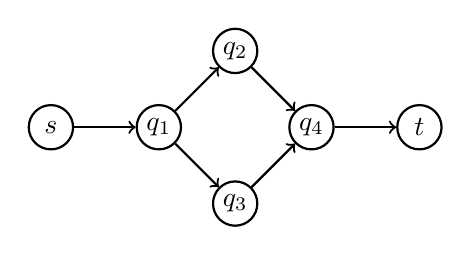
\begin{tikzpicture}[node distance={3.9em},
					thick, 
					main/.style = {draw, circle,fill=white, inner sep=1pt, minimum size=16pt}] 
					
					\node[main] (1) {$q_1$}; 
					\node[main] (2) [above right of=1] {$q_2$}; 
					\node[main] (3) [below right of=1] {$q_3$}; 
					\node[main] (4) [above right of=3] {$q_4$};
					\node[main] (5) [right of=4] {$t$}; 
					\node[main] (0) [left of=1] {$s$}; 
					\draw[->] (1) -- (2);
					\draw[->] (1) -- (3);
					\draw[->] (2) -- (4); 
					\draw[->] (3) -- (4); 
					\draw[->] (4) -- (5); 
					\draw[->] (0) -- (1);
				\end{tikzpicture}  
			\end{minipage}\hfill%
			\begin{minipage}[c]{0.64\textwidth}
				\begin{tikzpicture}[
					node distance={5.8em}, thick, 
					main/.style = {draw, rectangle, rounded corners=0.05cm,
						blur shadow, fill=white, inner sep=2pt, minimum size=13pt}
					]
					
					\node[main] (q1_eps) {$(q_1, \varepsilon)$}; 
					\node[main, fill=gray!30] (q1_b) [below right of=q1_eps] {$(q_1,b)$};
					
					\node[main] (q2_eps) [above right of=q1_eps]  {$(q_2,\varepsilon)$}; 
					\node[main, fill=gray!30] (q2_b) [below right of=q2_eps] {$(q_2,b)$};
					
					\node[main] (q3_eps) [below right of=q1_b] {$(q_3,\varepsilon)$}; 
					\node[main, fill=gray!30] (q3_b) [below right of=q3_eps] {$(q_3,b)$};
					
					\node[main] (q4_eps) [above right of=q3_eps] {$(q_4,\varepsilon)$};
					\node[main, fill=gray!30] (q4_b) [below right of=q4_eps] {$(q_4,b)$};
					
					\node[main, above right of=q4_eps] (t_eps) {$(t,\varepsilon)$};
					\node[main] (s_eps) [left of=q1_eps, xshift=0.3cm] {$(s,\varepsilon)$};
					
					\path[->] 
					(q1_eps)  edge [below,pos=.3] node {$b$} (q1_b)
					(q1_eps)  edge [left] node {$a$} (q2_eps)
					(q1_b)    edge [below,pos=.3] node {$a$} (q3_eps)
					(q1_b)    edge [out=180,in=290,above] node {$b$} (s_eps);
					
					\path[->] 
					(q2_eps) edge [out=280,in=175,below] node {$a$} (q4_eps)
					(q2_eps) edge [above,pos=.6] node {$b$} (q2_b)
					(q2_b)   edge [above,pos=.6] node {$a$} (q4_eps);
					
					\path[->] 
					(q4_eps) edge [left] node {$a$} (t_eps)
					(q4_eps) edge [left,pos=.5] node {$b$} (q4_b)
					(q4_b)   edge [left] node {$a$} (t_eps);
					
					% Koordinaten für Rücksprünge
					\coordinate (C) at ($(q4_b)+(0,-1.8)$);
					\coordinate (D) at ($(q2_b)+(0,1.8)$);
					
					\draw[->, rounded corners] 
					(q2_b) -- (D) -- (s_eps |- D) node[midway, above] {$b$} -- (s_eps);
					
					\draw[->, rounded corners] 
					(q4_b) -- (C) -- (s_eps |- C) node[midway, above] {$b$} -- (s_eps);
					
					\path[->] 
					(q3_eps) edge [above,pos=0.3] node {$a$} (q4_eps)
					(q3_eps) edge [below,pos=0.3] node {$b$} (q3_b)
					(q3_b)   edge [left] node {$a$} (q4_eps)
					(q3_b)   edge [out=180,in=280,above] node {$b$} (s_eps);
					
					\path[->] 
					(s_eps) edge node [above] {$a$} (q1_eps)
					(s_eps) edge [out=140, in=120, looseness=8, above] node {$b$} (s_eps);
					
					\path[->] 
					(t_eps) edge [loop above] node {$a,b$} (t_eps);
				\end{tikzpicture}
			\end{minipage}
			\caption[Example for reduction used in the proof of Prop.~\ref{prelim:prop:sync_NL_complete}]{Example for the reduction used in \cref{prelim:prop:sync_NL_complete}. Left: Input graph. Right: Transformation into an automaton having a synchronizing word if and only if there exists a path from $s$ to $t$ in the input graph (states from $V \times \{b\}$ are colored grey).}
			\label{prelim:fig:sync_NL_hard}
		\end{figure}
	
	\medskip 
	\noindent\underline{Properties:} The following two properties are readily seen.
	\begin{enumerate}
		\item \label{prelim:synctrap:bb} 
		$\applytrans{\delta}{Q \setminus \{(t,\varepsilon)\}}{bb} = \{(s,\varepsilon)\}$
		and  $\applytrans{\delta}{(t, \varepsilon)}{bb} = (t,\varepsilon)$.		
		
		\item \label{prelim:synctrap:transition} For $q \in V \setminus \{s,t\}$ 
		we have $\applytrans{\delta}{(q, \varepsilon)}{a} = (q^R,\varepsilon)$
		and $\applytrans{\delta}{(q, \varepsilon)}{ba} = (q^L,\varepsilon)$.
	\end{enumerate}
	
	\medskip 
	\noindent\underline{Verification:} First, suppose there exists a path $q_0, q_1, \ldots, q_n$
	with $q_0 = s$ and $q_n = t$ in $G$.
	Define a word $u = u_1 u_2 \cdots u_n$ 
	where $u_1 = a$ and, for $i \in \{2,\ldots,n\}$, 
	\[
	u_i = \begin{cases}
		a   & \text{if } q_i = q_{i-1}^R, \\
		ba	& \text{if } q_{i-1}^R \ne q_{i-1}^L \text{ and } q_i = q_{i-1}^L. 	
	\end{cases}
	\]	
	By Properties~\ref{prelim:synctrap:bb} and~\ref{prelim:synctrap:transition}, 
	$\applytrans{\delta}{Q}{bbu_1 \cdots u_i} = \{ (q_i,\varepsilon), (t,\varepsilon) \}$.
	So $\delta(Q,bbu) = \{(t,\varepsilon)\}$.		
	
	Conversely, suppose the word $u \in \Sigma^*$
	synchronizes $\mathcal A$.
	As $(t,\varepsilon)$ is a trap state, we have $\applytrans{\delta}{Q}{u} = \{(t,\varepsilon)\}$.
	Let $w$ be a shortest factor of $u$ such that $\delta((s,\varepsilon), w) = (t,\varepsilon)$.
	By Property~\ref{prelim:synctrap:bb} we have $w \notin \Sigma^* bb \Sigma^*$, i.e., 
	$w \in \{a,ba\}^* \cup \{a,ba\}^*b$.
	As we can enter the state $(t,\varepsilon)$ from another state only via the letter~$a$,
	we have $w \in \{a,ba\}^*$. 
	Let $w = w_1 \cdots w_n$ with 
	$w_1, \ldots, w_n \in \{a,ba\}^*$.
	Then, by Property~\ref{prelim:synctrap:transition}, the vertices
	\[
	(s,\varepsilon), \applytrans{\delta}{s}{w_1}, \applytrans{\delta}{s}{w_1 w_2} \ldots
	\applytrans{\delta}{s}{w_1 w_2\cdots w_{n-1}}, (t,\varepsilon) 
	\]
	trace out a path in $G$ from $s$ to $t$.		
\end{proof} 

\begin{proposition}\label{prelim:complexity:prop:maximum}
	Given an automaton $\semiautomat{A}{Q}{\Sigma}{\delta}$ and $q \in Q$
	it is \NL-complete to test whether $q$ is a maximum w.r.t.~the 
	reachability quasiorder $\lereach$.	
\end{proposition}
\begin{proof}
	First, we give
	an $\leACZEROm$-reduction from \DFAST, which yields \NL-hardness by \PROP~\ref{prelim:prop:sync_NL_complete}.
	Let $\semiautomat{A}{Q}{\Sigma}{\delta}$
	be an input instance to \DFAST.
	Suppose $t \in Q$ is the trap state, which 
	can be computed by an $\AC^0$-circuit as 
	in the proof of \crefitem{compl:prop:reductions}{compl:prop:reductions:item:st-ss}.
	So, the reduction produces $\mathcal A$ together with the trap state~$t$
	and $(\mathcal A, t)$ is a {\sc Yes}-instance of our problem
	if and only if $\mathcal A$ is synchronizing,
	since the state $t$ is a maximum in $\mathcal A$
	if and only if~$\mathcal A$ is synchronizing by \cref{prelim:thm:sync_trap_state}.
		
	For containment in \NL, suppose $\semiautomat{A}{Q}{\Sigma}{\delta}$ and $q \in Q$
	are given.
	To test whether $q$ is a maximum for $\lereach$,
	we guess, for each state $p \in Q$,
	a word $u \in \Sigma^{<|Q|}$
	letter by letter and check whether $\applytrans{\delta}{p}{u} = q$; a property that characterizes that~$q$ is a maximum
	by \cref{prelim:classes:sync:cor:sync-state}.
	This can be 
	done in nondeterministic log-space
	by storing a state
	and using two counters, one to iterate through all states $p \in Q$
	and the other to make at most $|Q|$ guessing steps for each $p \in Q$.	
\end{proof}

\begin{proposition}\label{prelim:complexity:prop:maximal}
	Given an automaton $\semiautomat{A}{Q}{\Sigma}{\delta}$ and $q \in Q$
	it is \NL-complete to test whether $q$ is maximal w.r.t.~the 
	reachability quasiorder $\lereach$.	
\end{proposition}
\begin{proof}
	We give a reduction
	from the \NL-complete problem \TWODAGST.
	Let $G = (V, E)$ and $s, t \in V$ be an input instance.
	Construct an automaton $\semiautomat{A}{Q}{\Sigma}{\delta}$
	as in the proof of \cref{prelim:prop:sync_NL_complete},
	but instead of making $(t,\varepsilon)$ a trap state,
	let both letters $a$ and $b$ map back to the state $(s,\varepsilon)$.
	Then $t$ is a maximal state (and~$\mathcal A$
	is strongly connected) if and only if there exists
	a path from~$s$ to $t$ in~$G$.
		
	To test maximality, we have to check
	that for each state $p \in Q$
	with $\delta(q, u) = p$ for some $u \in \Sigma^*$
	there exists $v \in \Sigma^*$
	with $\delta(p, v) = q$.
	To verify this condition, we can pick words $u,v$
	of length at most $|Q|$
	and proceed similarly as in the proof of \cref{prelim:complexity:prop:maximum}
	to obtain \NL-membership.	
\end{proof}

Similar procedures as in \cref{prelim:complexity:prop:maximum,prelim:complexity:prop:maximal}
can be used to check whether a state is minimal or a minimum, but we do not need to check these properties
in the following and hence give no formal statement. We also note that we obtain
\LOGSPACE-completeness of these problems in case the input automata are unary automata
since we only needed nondeterminism when guessing different letters in the above proofs.

\begin{theorem}\label{prelim:complexity:general_aut_sync}
	The problems \DFAS, \DFAST and \DFASS
	are \NL-complete, even for a fixed binary alphabet.
\end{theorem}
\begin{proof} 
	By Proposition~\ref{compl:prop:reductions} 
	we have $\DFAST \leACZEROm \DFASS$
	and $\DFAST \leACZEROm \DFAS$.
	By \cref{prelim:prop:sync_NL_complete}, \DFAST\   %can be solved by an \NL-algorithm % fussnote alternative paare auf q
	is \NL-hard for an alphabet containing at least two letters.
	\DFAS\ is in \NL, see \cref{compl:sec:subclasses:known-results} (page~\pageref{prelim:classes:intro:SYNC}).
	For $\semiautomat{A}{Q}{\Sigma}{\delta}$, by \THM~\ref{prelim:thm:SCC_sync_words},
	a state $q \in Q$
	is a synchronizing state if and only if $\mathcal A$ is synchronizing and $q$ is
	a maximum for the reachability order $\lereach$.
	The latter two properties can be checked in \NL\  since \DFAS\ is in \NL and by~\cref{prelim:complexity:prop:maximum}, respectively.
	So, \DFASS is in~\NL.	
\end{proof}

\begin{proposition}\label{prelim:thm:ST-PSPACE}
	\ST is in \PSPACE.
\end{proposition}
\begin{proof}
	Let $(\mathcal A, S, T)$ with $\semiautomat{A}{Q}{\Sigma}{\delta}$
	and $S, T \subseteq Q$ where $S = \{s_1, \ldots, s_m\}$ and $n = |Q|$.
	Store the values $s_1, \ldots, s_m$ in $m$ memory cells
	and then repeat the following steps
	at most~$n^m$ times:  
	If the memory cells store a subset of~$T$, then abort and return \rYES, i.e., classify 
	this input instance as a \rYES-instance of the decision problem.
	Otherwise
	guess a letter $a \in \Sigma$ and update the memory cells
	with $\applytrans{\delta}{s_1}{a}, \ldots, \applytrans{\delta}{s_m}{a}$.
	If this procedure finishes without ever writing a subset of~$T$ into the memory cells, 
	then return \rNO.
	The upper bound for the number of steps
	can be ensured by utilizing an  $(m\cdot \log n)$-bit counter 
	counting the number of steps in binary encoding.
	After at most $n^m$
	steps we have seen at least one memory cell configuration twice.
	So, if there exists a word mapping $S$ into $T$, then
	there exists such a word of length at most $n^m$,
	which implies correctness of the algorithm.
	As it runs in nondeterministic polynomial space,
	and as \PSPACE\  = \NPSPACE\ by Savitch's theorem~\cite{DBLP:journals/jcss/Savitch70},
	the claim follows.
\end{proof}

The following lemma is a technical result that we need to reduce an arbitrary alphabet to a binary alphabet
in our subset mapping problems.
Another reduction to reduce the alphabet for synchronization problems has been given
in~\cite[Sec.~5]{Martyugin12} and~\cite[Prop.~2]{Martyugin14}.


\begin{lemma} \label{prelim:lem:alphabet-reduction}
	Let $\semiautomat{A}{Q}{\Sigma}{\delta}$ with $\Sigma = \{a_1, \ldots, a_k\}$.
	Set $C = \{ 0^{k} 10^i1 \mid i \in \{0,1,\ldots,k-1\}\}$
	and $\semiautomat{B}{Q \times \pref{C}\setminus C}{\{a,b\}}{\mu}$
	where, for $q \in Q$, $u \in \pref{C}\setminus C$, and $x \in \{a,b\}$,
	we have
	\[
	\mu((q,u), x) =
	\begin{cases}
		(\delta(q, a_i), \varepsilon) & \text{if } ux = 0^k10^{i-1}1 \text{ for some } i \in \{1,\ldots,k\}, \\
		(q, ux)  & \text{if } ux \in \pref{C} \setminus C, \\
		(q, ux)  & \text{if } u \in \pref{0^{k-1}} \text{ and } x = 0, \\
		(q, 0^k) & \text{if } u = 0^k \text{ and } x = 0, \\
		(q, 0^k) & \text{if } u = 0^k10^{k-1} \text{ and } x = 0, \\
		(q, \varepsilon) & \text{otherwise.}
	\end{cases}
	\]
	Then $\mathcal A$ is strongly connected if and only if $\mathcal B$ 
	is strongly connected and, for $i \in \{1,\ldots,k\}$, $q \in Q$, $u \in \pref{C}\setminus C$,
	we have
	\begin{equation}\label{prelim:eqn:general-to-binary}
	\mu((q, u), 0^k10^{i-1}1) = (\delta(q, a_i), \varepsilon),
	\end{equation}
	and, for distinct $S, T \subseteq Q$,
	we have $\delta(S, u) = T$ for some $u \in \Sigma^*$
	if and only if $\mu(S \times \pref{C}\setminus C, v) = T \times \{\varepsilon\}$ 
	for some $u \in \{a,b\}^*$.
\end{lemma}
\begin{proof}
	That~$\mathcal A$ is strongly connected if and only if~$\mathcal B$
	is strongly connected is easy to see.
	\Cref{prelim:eqn:general-to-binary} is also easy to verify.
		
 Next, suppose $\delta(S, u) = T$ for some $u \in \Sigma^*$. Since $S \ne T$ we have $|u| > 0$.
 Let $v_j = 0^k 1 0^{i-1} 1$ if the $j$-th symbol in~$u$ equals $a_i$
 for $i \in \{1,\ldots,k\}$.
 By \cref{prelim:eqn:general-to-binary} 
 we have $\mu(S \times \pref{C}\setminus C, v_1 \cdots v_{|u|}) = (T, \varepsilon)$.
 
 Conversely, suppose $\mu(S \times \pref{C}\setminus C, v) = T \times \{\varepsilon\}$ 
 for some $u \in \{a,b\}^*$.
 Let $q \in S$ and $u \in \pref{C}\setminus C$.
 The language~$C$ has the property that there exist unique words
 $u_1, \ldots, u_m \in C$ and $v_0, \ldots, v_m \in \Sigma^*$,
 each $v_j$ containing no factor from~$C$, such that
 \[
 uv = v_0 u_1 v_1 \cdots u_m v_m.
 \]
 For each $j \in \{1,\ldots,m\}$, set $x_j=a_i$ if
 $u_j = 0^k10^{i-1}1$ for some $i \in \{1,\ldots,k\}$.
 By induction, using \cref{prelim:eqn:general-to-binary}, we obtain
 \[
 \mu((q,u),v)
 =
 (\delta(q,x_1\cdots x_m),\varepsilon).
 \]
 Hence $\delta(S,x_1\cdots x_m)=T$. 
\end{proof}

\begin{theorem}\label{prelim:thm:binary_pspace_problems} The following problems are \PSPACE-complete w.r.t.~$\lelogm$-reductions:
	\begin{enumerate}
		\item \SFS and \SIS even on binary strongly connected  automata,
		\item \DFAINT, \ST, and \DST even on binary strongly connected  automata,
		\item \REACH and \REACHF even for binary automata.
	\end{enumerate}
\end{theorem}
\begin{proof}
	Membership of these problems in \PSPACE\ was 
	proved in the literature, see  \cref{compl:sec:subclasses:known-results} (page~\pageref{prelim:classes:intro:SFS}).
	As an example, we included a proof
	for \ST in \cref{prelim:thm:ST-PSPACE}.
	
	\PSPACE-hardness of \SFS and \SIS for binary strongly connected automata
	was also mentioned  in \cref{compl:sec:subclasses:known-results} (page~\pageref{prelim:classes:intro:SFS}).
	
	By \cref{compl:prop:reductions} we have
	\[
	\SIS \leACZEROm \ST \leACZEROm \DFAINT
	\]
	and the reductions from \cref{compl:prop:reductions}
	preserve strong connectedness and the alphabet.
	Thus, the claim for \ST and \DFAINT follow.
	
	The reduction showing $\ST \leACZEROm \DFAINT$
	from \cref{compl:prop:reductions:item:DFAINT_ST} in \cref{compl:prop:reductions}
	does not preserve strong connectedness and the alphabet.
	However, it can easily be adapted 
	by adding a new letter that swaps two states $q$ and $(q,0)$ 
	with $q \in S$
	and induces a self-loop at every other state not in~$S$.
	Then the resulting automaton is strongly connected
	and this gives a valid reduction.
	With \cref{prelim:lem:alphabet-reduction} 
	we then obtain \PSPACE-hardness
	even for binary strongly connected automata.
	This proves the claim for \DFAINT, \ST, and \DST.
	
	\REACH was shown to be \PSPACE-hard
	in~\cite[Thm.~3.2]{Rys83}
	and~\cite[Thm.~3]{BondarV16}
	by reductions from  
	\SIS and \DFAINT, respectively,
	that add a single new letter.
	Neither of these reductions preserves strong connectedness.
	By \cref{prelim:lem:alphabet-reduction}	we obtain a reduction 
	to a binary alphabet.
	Since $\REACH \leACZEROm \REACHF$
	by \cref{compl:prop:reductions}
	where the reduction preserves the alphabet,
	we obtain the hardness claims for \REACH and \REACHF.
\end{proof}

\subsection{Solvable Automata}
\label{compl:sec:solv} 

%!TEX root = ./../../springer-mono-format/book.tex
%!TEX root = ./../../thesis-trier.tex

Here, we show the following:

\begin{enumerate}
	\item \ST, \DST, and \DFAINT are \NP-complete for solvable input automata
	(\cref{thm:solvable}).
	
	\item \SFS is \NP-complete for solvable automata (\cref{thm:SF-solvable}).
	
	\item \DFAST, \DFASS, \DFAS, and \SIS are \LOGSPACE-complete
	for solvable automata even for a unary alphabet (\cref{thm:SYNC-solv}).
	
	\item \REACHF and \REACH are \NP-complete for solvable automata
	in (\cref{prelim:compl:thm:reach-NP,prelim:compl:thm:reachf-NP}).
\end{enumerate}
For self-containment, we give a proof of \NP-hardness of \DFAINT 
for unary permutation automata. The proof is similar to the one given in \cite[Lem.~27]{MartensN07},
but uses automata instead of regular expressions.

\begin{proposition}
	\label{compl:prop:dfaint_unary}
	\DFAINT is \NP-hard for unary permutation automata.
\end{proposition}
\begin{proof}	
	We give a reduction from {\sc 3SAT}, which 
	is \NP-complete by \cref{prelim:thm:THREESAT}.
	Let $C_1, \ldots, C_m \subseteq \{x_1, \overline x_1, \ldots, x_n, \overline x_n\}$ 
	be the clauses of an {\sc 3SAT}-instance over the variables $x_1, \ldots, x_n$.
	We can assume every variable appears, as a positive or negative literal, in some clause.
	
	\medskip 
	\noindent\underline{Construction:} 
	Let $p_1 < p_2 < \cdots < p_n$
	be the first $n$ prime numbers.
	For each clause $C_j$, $j \in \{1,\ldots,m\}$,
	we construct 
	$\automat{A_j}{Q_j}{\{a\}}{\delta_j}{q_j}{F_j}$
	with
	\begin{align*}
		Q_j & = \{0,1,\ldots, N_j - 1\}, \\
		q_j & = 0, \\
		F_j & = \{ q \in Q_j \mid \exists i \in \{1,\ldots,n\} : 
		( x_i \in C_j \land q \equiv_{p_i} 0 ) \lor ( \overline{x}_i \in C_j \land q \not\equiv_{p_i} 0 ) \}, \\
		%F_j & = \{ q \in Q_j \mid \exists i \in \{1,\ldots,n\} : 
		%( x_i \in C_j \land q \equiv 0 \pmod{p_i} ) \\ 
		%& \qquad\qquad\qquad\qquad\qquad\qquad\qquad \lor ( \overline{x}_i \in C_j \land q \not\equiv 0 \pmod{p_i}) \}, \\
		\applytrans{\delta_j}{q}{a} & = (q + 1) \bmod{ N_j }
	\end{align*}
	where $N_j = \left(\prod_{\substack{ i \in \{1,\ldots,n\} \\ x_i \in C_j \lor \overline{x}_i \in C_j}} p_i \right)$,
	i.e., we multiply those primes that correspond
	to the variables in~$C_j$.
	
	By \cref{prelim:cor:PNT} 
	there exists $N \ge 1$ such that $p_n < n^2$
	for all $n \ge N$.
	We can assume $p_n < n^2$ in the following.
	Since  $|C_j| \le 3$
	we get  $|Q_j| \le n^6$.
	Then, as detecting primality for unary numbers
	is in~\LOGSPACE~\cite[Thm.~7]{DBLP:journals/tcs/HartmanisB76},
	the automata $\mathcal A_j$ can be constructed 
	in deterministic log-space.	
	
	\Cref{prelim:compl:fig:intersection-unary-construction} 
	shows the construction for the clauses $C_1 = \{ x_1, x_2\}$, $C_2 = \{ \overline{x_1}, x_3\}$,
	and $C_3 = \{ x_2, \overline{x_3}\}$ (shown in their logical interpretation
	in the figure).
	If $x_1 = 1$, then $x_3 = 1$ to fulfill $C_2$
	and thus $x_2 = 1$ to fulfill $C_3$. For $x_1 = 0$,
	we must have $x_2 = 1$ to fulfill $C_1$
	and $x_3$ can be arbitrary. Thus we find 
	three satisfying assignments that correspond to 
	the words $a^{30}$, $a^3$, and $a^{15}$.	
	
	\begin{figure}[ht]
		\centering	
		
		\begin{tikzpicture}[>=Stealth] %[>=Stealth[length=3pt]] %
			
			% ---------- Stil & Radius ----------
			\def\radius{11em}
			\def\radiusA{0.3*\radius}
			\def\radiusB{0.44*\radius}
			\def\radiusC{0.67*\radius}
			\def\ylabel{\radiusC-2em}
			
			\tikzset{
				smallstate/.style={
					draw,
					circle,
					minimum size=15pt,
					inner sep=0pt,
					font=\small
				}
			}
			
			% ---------- Automat mit 6 Zuständen ----------
			\begin{scope}
				\foreach \i in {0,...,5} {
					% teilbar durch 2 ODER 3
					\pgfmathtruncatemacro{\isfinal}{(mod(\i,2)==0) || (mod(\i,3)==0)}
					\ifnum\isfinal=1
					\node[smallstate,accepting] (q\i) at ({360/6*\i}:\radiusA) {$\i$};
					\else
					\node[smallstate] (q\i) at ({360/6*\i}:\radiusA) {$\i$};
					\fi
				}
				\foreach \i in {0,...,5} {
					\pgfmathtruncatemacro{\j}{mod(\i+1,6)}
					\draw[->] (q\i) edge (q\j);
				}
				\node at (0,-\ylabel) {$\mathcal A_1$ for $C_1 = x_1 \lor x_2$};
			\end{scope}
			
			% ---------- Automat mit 10 Zuständen ----------
			\begin{scope}[xshift=12em]
				\foreach \i in {0,...,9} {
					% ungerade UND durch 3 teilbar
					\pgfmathtruncatemacro{\isfinal}{(mod(\i,2)==1) || (mod(\i,5)==0)}
					\ifnum\isfinal=1
					\node[smallstate,accepting] (p\i) at ({360/10*\i}:\radiusB) {$\i$};
					\else
					\node[smallstate] (p\i) at ({360/10*\i}:\radiusB) {$\i$};
					\fi
				}
				\foreach \i in {0,...,9} {
					\pgfmathtruncatemacro{\j}{mod(\i+1,10)}
					\draw[->] (p\i) edge (p\j);
				}
				\node at (0,-\ylabel) {$\mathcal A_2$ for $C_2 = \overline{x_1} \lor x_3$};
			\end{scope}
			
			% ---------- Automat mit 15 Zuständen ----------
			\begin{scope}[xshift=28em]
				\foreach \i in {0,...,14} {
					% gerade UND NICHT durch 5 teilbar
					\pgfmathtruncatemacro{\isfinal}{(mod(\i,2)==0) || (mod(\i,5)!=0)}
					\ifnum\isfinal=1
					\node[smallstate,accepting] (r\i) at ({360/15*\i}:\radiusC) {${\i}$};
					\else
					\node[smallstate] (r\i) at ({360/15*\i}:\radiusC) {${\i}$};
					\fi
				}
				\foreach \i in {0,...,14} {
					\pgfmathtruncatemacro{\j}{mod(\i+1,15)}
					\draw[->] (r\i) edge (r\j);
				}
				\node at (0,-\ylabel) {$\mathcal A_3$ for $C_3 = x_2 \lor \overline{x_3}$};
			\end{scope}	
		\end{tikzpicture}
		\caption[Example for reduction of \THREESAT to \DFAINT\ on unary automata]{Example for the proof of \cref{compl:prop:dfaint_unary}. States with label~$0$ are start states. Final states are indicated by double circles. The label~$a$ at the transitions is omitted.}
		\label{prelim:compl:fig:intersection-unary-construction}
	\end{figure} 
		
	\medskip
	\noindent\underline{Properties:} We have the following two properties:
	\begin{enumerate}
		\item \label{prelim:compl:INT-unary:1} $\delta_j(q_j, a^r) \equiv_{N_j} r$ for each $r \ge 0$.
		
		\item \label{prelim:compl:INT-unary:2} $(b_1, \ldots, b_n)$ is a satisfying assignment
		if and only if $a^{\prod_{i=1}^n p_i^{b_i}} \in \bigcap_{j=1}^m L(\mathcal A_j)$.
	\end{enumerate}	
	Property~\ref{prelim:compl:INT-unary:1} follows 
	from the construction of $\mathcal A_j$ whose automaton graph forms a single cycle.	
	Property~\ref{prelim:compl:INT-unary:2} follows since for $(b_1, \ldots, b_n) \in \{0,1\}^n$,
	$l = \prod_{i=1}^n p_i^{b_i}$,  $j \in \{1,\ldots,m\}$,
	and $s_j = \delta_j(q_j, a^l)$ we have $s_j \equiv l \pmod{N_j}$ and then
	\[
	\begin{array}{rlr}
		&\exists i \in I \colon ( ( x_i \in C_j \land b_i = 1 ) \lor ( \overline{x}_i \in C_j \land b_i = 0 ) ) \\
		& \Leftrightarrow \exists i \in I \colon ( ( x_i \in C_j \land l \equiv_{p_i} 0 ) \lor ( \overline{x}_i \in C_j \land l \not\equiv_{p_i} 0  ) )  & \text{(Def. $l$)} \\
		& \Leftrightarrow  \exists i \in I \colon( ( x_i \in C_j \land s_j \equiv_{p_i} 0 ) \lor ( \overline{x}_i \in C_j \land s_j \not\equiv_{p_i} 0 ) ) & \text{(Eqn.~\eqref{prelim:eqn:ab_divisor}, Property~(1))} \\
		& \Leftrightarrow  s_j \in F_j & \text{(Def. $F_j$)}
	\end{array}
	\]
	where $I = \{1,\ldots,n\}$.
	
	\medskip 
	\noindent\underline{Verification:} By Property~\ref{prelim:compl:INT-unary:2},
	if there exists a satisfying assignment, then we have $\bigcap_{j=1}^m L(\mathcal A_j) \ne \emptyset$.
	Conversely, suppose $a^l \in \bigcap_{j=1}^m L(\mathcal A_j)$
	for some $l \ge 0$. Define an assignment $(b_1, \ldots, b_n)$
	to the variables by setting, for $i \in \{1,\ldots,n\}$,
	\[
	b_i = \begin{cases}
		1 & \text{if } p_i \text{ divides } l, \\ 
		0 & \text{if } p_i \text{ does not divide } l. 
	\end{cases}	
	\] 	
	Let $l' = \prod_{i=1}^n p_i^{b_i}$.
	Then $l' \equiv_{p_i} 0$ if and only if $l \equiv_{p_i} 0$ for $i \in \{1,\ldots,n\}$.
	So $a^{l'} \in L(\mathcal A_j)$ if and only if $a^l \in L(\mathcal A_j)$ for $j \in \{1,\ldots,m\}$.
	Hence, by Property~\ref{prelim:compl:INT-unary:2}, we obtain that $(b_1, \ldots, b_n)$
	is a satisfying assignment.
\end{proof}

\begin{theorem}\label{thm:solvable} \label{compl:thm:comm_ST}
	\ST, \DST, and \DFAINT are \NP-complete for solvable input automata,
	where \NP-hardness holds
	even for the following classes of input automata:
	\begin{enumerate}
		\item binary partially ordered input automata,
		
		\item ternary partially ordered monotonic automata,
		
		\item commutative partially ordered  automata over an unbounded alphabet,
		
		\item unary permutation automata.
	\end{enumerate}
\end{theorem}
\begin{proof}
	That \DFAINT is \NP-complete for the mentioned
    classes follows from results
    in the literature mentioned in \cref{compl:sec:subclasses:known-results}, page~\pageref{prelim:classes:intro:INT}.
    By \cref{compl:prop:reductions:item:DFAINT_DST,compl:prop:reductions:item:DST_ST}
    from \cref{compl:prop:reductions} 
    we obtain \NP-hardness for all three problems,
    and by these statements it is sufficient to establish \NP-membership
    for \ST, which we do in the following.
    
	Let $\Sigma = \{a_1, \ldots, a_k\}$ and 
	$\semiautomat{A}{Q}{\Sigma}{\delta}$ be a solvable
	input automaton to \ST with $n$ states and input sets $S, T \subseteq Q$.
	If there exists a word mapping~$S$ into~$T$,
	by Proposition~\ref{prop:S-T-bound} there exists a word
	of the form
	\[ 
	v = v_0 x_1 \cdots v_{r-1} x_r v_r
	\]
	for some $r \le n^2$
	where $x_1, \ldots, x_r \in \Sigma$ and $v_i = a_1^{r_{i,1}} \cdots a_k^{r_{i,k}}$
	for numbers $0 \le r_{i,j} < 2^n$
	with $i \in \{0,1,\ldots,r\}$ and $j \in \{1,\ldots,k\}$
	mapping~$S$ into~$T$.
	By using a binary encoding for the exponents $0 \le r_{i,j} < 2^n$,
	a word of the above form can be stored using 
	$O( |\Sigma|n \cdot (n^2 + 1) + \log(|\Sigma|)n^2)$
	%$(|\Sigma|+1) n^3 + |\Sigma|n$ 
	bits where each of the $n^2+1$ words $v_i$, $i \in \{0,1,\ldots,r\}$,
	takes up $|\Sigma|n$ bits and each letter $x_i$, $i \in \{1,\ldots,r\}$,
	takes $\log( |\Sigma| )$ bits.
	So, using this encoding, it can be guessed in polynomial time.
	Next, the transition matrix
	of $a_j^{r_{i,j}}$ for $0 \le r_{i,j} < 2^n$
	can be computed in polynomial time by a square-and-multiply algorithm (also known as 
	exponentiation by squaring) 
	using the transition matrix of~$a_j$.
	Hence, the transition matrix of~$v$
	can be computed in polynomial time by multiplying
	the transition matrices of $v_0, x_1, \ldots, v_{r-1}, x_r$, and $v_r$ in this order.
	Then~$v$ maps~$S$ into~$T$
	if and only if each row in the transition matrix of~$v$ corresponding to a state in~$S$
	has precisely one~$1$ at a column corresponding to a state in~$T$.
	So, the above algorithm shows containment in \NP. 
\end{proof}

\begin{theorem}\label{thm:SF-solvable}
	\SFS is \NP-complete for solvable input automata even for binary partially ordered automata.
\end{theorem} 
\begin{proof}
	Ryzhikov~\cite[Thm.~4]{Ryzhikov19a} proved the problem to be \NP-complete
	for partially ordered binary automata, see also page~\pageref{prelim:classes:intro:SFS} 
	in \cref{compl:sec:subclasses:known-results}.
	
	For \NP-membership, we can guess a state $q \in Q$ in an $n$-state solvable 
	input automaton $\semiautomat{A}{Q}{\Sigma}{\delta}$
	and then test whether 
	there exists a word mapping $Q$ to $\{q\}$.
	As the latter problem is in \NP\  by Theorem~\ref{thm:solvable},
	we obtain that \SFS is in \NP. 
	\NP-hardness follows as \SFS
	is \NP-complete for binary partially ordered automata
	as proved in~\cite[Thm.~4]{Ryzhikov19a}, 
	see also Table~\ref{compl:tab:overview}.
\end{proof}

\begin{theorem} \label{thm:SYNC-solv}
\DFAST, \DFASS, \DFAS, and \SIS are \LOGSPACE-complete for solvable input automata, even for a fixed unary alphabet.
\end{theorem}
\begin{proof}
	By \cref{compl:prop:reductions} we have
	\[
	\SCP \leACZEROm \DFAST \leACZEROm  \DFASS \leACZEROm \SIS,
	\]
	and $\DFAST \leACZEROm \DFAS$,
	where the reductions of an automata-theoretical problem to another automata-theoretical problem given in the proof
	of \cref{compl:prop:reductions} preserve the alphabet.
	Since \SCP is \LOGSPACE-complete by \cref{prelim:thm:complexities},
	and the reduction to \DFAST 
	works even for unary automata, we obtain the \LOGSPACE-hardness claims even for a fixed unary alphabet.
	
	
	Since the reductions from \cref{compl:prop:reductions} transforming automata preserve
	the property of being solvable, 
	by the reductions from above, it is sufficient to prove \LOGSPACE-membership
	for \DFAS and \SIS to establish it for the other problems as well.
	
	For \DFAS, to test synchronizability, by Theorem~\ref{prelim:thm:solvrank_r} 
	we can simply test whether the word $(a_1 \cdots a_k)^{n-1}$ for $\Sigma = \{a_1, \ldots, a_k\}$
	synchronizes the $n$-state solvable input automaton, which can be done in deterministic log-space
	by Theorem~\ref{prelim:thm:finite_list_sync_word}.
	
	However, this is not sufficient since we cannot simply construct the word
	as this would take up more than logarithmic space, i.e.,
	having a deterministic log-space Turing machine 
	deciding whether a word synchronizes a given automaton,
	we cannot simply write $(a_1 \cdots a_k)^{n-1}$ and an encoding of the automaton 
	on its input tape and then simulate it, as this would
	take up more than logarithmic space.
	But we can simulate the machine by letting it read the input automaton
	from the original input tape
	and feeding
	$(a_1 \cdots a_k)^{n-1}$ one symbol at a time to it in log-space without storing the full word similarly as closure of \LOGSPACE
	is proved for log-space transducers, see~\cite[Lem.~13.2]{HopUll79}; in fact,
	a log-space transducer that additionally produces 
	$(a_1 \cdots a_k)^{n-1}$ can also be given to obtain the claim.
	% (the word \todo{satz in klammern geadded, 20.3}
	% $(a_1 \cdots a_k)^{n-1}$ cannot be stored in log-space, 
	% but it can be feed one symbol at a time to the other problem in log-space
	% similarly as closure of \LOGSPACE
	% is proved for log-space transducers, see~\cite[Lem.~13.2]{HopUll79}; in fact,
	% a log-space transducer that additionally produces 
	% $(a_1 \cdots a_k)^{n-1}$ can also be given to obtain the claim).	
		
	To solve \SIS for $\semiautomat{A}{Q}{\Sigma}{\delta}$ and $S \subseteq Q$, 
	by \crefitem{prelim:classes:solvable:thm}{prelim:prop:solvable-SCC:2}
	and \cref{prelim:classes:block:cor:Q-into-S}
we have to test whether~$S$ contains all sink components of~$\mathcal A$.
We can do this by iterating through all states $q \in Q$,
test whether it is contained in a sink component
and if this is the case, test whether $q \in S$.
By \cref{prelim:classes:block:prop:char-sink-state},
a state $q \in Q$
is in a sink component if and only if for all $x \in \Sigma$ 
we have $\delta(q, x^i) = q$ for some $i \in \{1,\ldots,|Q|\}$.
This can be checked in deterministic log-space
by successively applying~$|Q|$ times --- using a counter that counts 
up to~$|Q|$ and so takes up at most logarithmic space via a binary encoding --- the letter~$x$ to a state stored in 
a memory cell initialized with~$q$. Then it is easy to give an algorithm running
in deterministic log-space.
%and a counter that counts up to~$|Q|$ and, via a binary encoding, uses
%at most logarithmic space.	
\end{proof}

\begin{theorem} \label{prelim:compl:thm:reach-NP}
	\REACH is \NP-complete for solvable automata even for partially ordered binary automata.	
\end{theorem}
\begin{proof}
	The problem is \NP-complete for partially ordered binary
	automata~\cite[Thm.~5]{Ryzhikov19a}.
	Furthermore, as in the proof of Theorem~\ref{thm:solvable}
	by using Proposition~\ref{prop:S-T-bound}
	we obtain \NP-membership for solvable automata. 
\end{proof}

\begin{theorem} \label{prelim:compl:thm:reachf-NP}
	\REACHF is \NP-complete for solvable automata even for commutative partially ordered automata,
	and also even for partially ordered binary automata.
\end{theorem}
\begin{proof}
	\NP-hardness for partially ordered binary automata
	follows from \cref{prelim:compl:thm:reach-NP}
	and \cref{compl:prop:reductions:item:REACH-REACHF} from \cref{compl:prop:reductions}.
	Next, in~\cite[Thm.~9]{DBLP:journals/iandc/Beaudry88}
	it has been shown that deciding
	for commutative partially ordered $\mathcal A = (Q, \Sigma, \delta)$
	and $t \colon Q \to Q$
	whether there exists $u \in \Sigma^*$
	such that $\delta(q, u) = t(q)$
	for all $q \in Q$ is \NP-complete.\footnote{In~\cite{DBLP:journals/iandc/Beaudry88} this problem was formulated as a problem on transformation monoids, where the 
		commutative aperiodic transformation monoids used
		correspond precisely to the commutative partially ordered automata.}
	This problem can be reduced to \DFAINT 
	by letting $Q = \{q_1, \ldots, q_n\}$ and $\mathcal A_i = \mathcal A$
	and $F_i = \{t(q_i)\}$ for $ i \in \{1,\ldots,n\}$.
	Then when applying the reduction
	from \crefitem{compl:prop:reductions}{compl:prop:reductions:item:DFAINT_DST}
	 to obtain an instance of \ST 
	from this \DFAINT-instance
    the resulting automaton is a commutative partially ordered automaton 
	$\mathcal A' = (Q', \Sigma, \delta')$
	where $\delta'(\{q_1, \ldots, q_n\}, u) \subseteq F_1 \cup \ldots \cup F_n$
	if and only if $\delta'(\{q_1, \ldots, q_n\}, u) = F_1 \cup \ldots \cup F_n$ for $u \in \Sigma^*$, i.e., we actually have a reduction to \REACHF.
	
	As in the proof of Theorem~\ref{thm:solvable},
	by using Proposition~\ref{prop:S-T-bound},
	we obtain that \REACHF is in \NP\ 
	for solvable automata.
\end{proof}

\subsection{Commutative Automata}
\label{comp:sec:comm}

%!TEX root = ./../../springer-mono-format/book.tex
%!TEX root = ./../../thesis-trier.tex

Here, we show the following:
\begin{enumerate}
\item \DFAINT, \DST, and \ST are \LOGSPACE-completeness for partially ordered commutative automata
over a fixed non-empty alphabet (\cref{thm:SF-ST-comm}).
Recall that in \cref{compl:sec:solv} we have shown that these problems
are \NP-complete for partially ordered commutative automata over an unbounded alphabet.

\item \SFS is \LOGSPACE-complete for commutative automata (\cref{thm:SF-ST-comm})
even for unary partially ordered automata. Recall that this problem is \NP-complete
for solvable automata by \cref{thm:SF-solvable}.

\item \DFASWS\ is \LOGSPACE-complete for commutative automata over a fixed alphabet 
and \NP-complete for an unbounded alphabet (\cref{compl:thm:comm-syncshort}).
Hardness remains in both cases even for partially ordered commutative automata.
\end{enumerate}

In this section, we assume an ordering $\Sigma = \{a_1, \ldots, a_k\}$ of each input alphabet~$\Sigma$
with $k \ge 1$ (the case $\Sigma = \emptyset$ is trivial and most problems are solvable in constant time).

\begin{theorem}\label{thm:SF-ST-comm}
	\begin{enumerate}		
		\item \SFS is \LOGSPACE-complete for commutative automata over an unbounded alphabet, where \LOGSPACE-hardness holds even for unary partially ordered automata.
		
		\item \ST, \DST, \DFAINT are \LOGSPACE-complete for partially ordered commutative automata over a fixed non-empty alphabet
		even for an alphabet of size one.
	\end{enumerate}
\end{theorem}
\begin{proof}
	By \cref{compl:prop:reductions},
	where the reductions preserve
	the properties of commutativity, partial orderness,
	and the alphabet,
	it is sufficient to show the second claim for \ST.	
	
	For hardness, we give a reduction from \ONEDAGST that works for \SFS 
	and \ST, and also even if we fix $k$ to be equal to one. 
	For an \ONEDAG-instance $(G, s, t)$ with $G = (V,E)$,
	let $\semiautomat{A}{V}{\Sigma}{\delta}$
	where, for $p \in V$ and $x \in \Sigma$, 
	\[
	\delta(p, x) = \begin{cases}
		q & \text{if } (p,q) \in E \text{ for some } q\in V, \\
		p & \text{otherwise.}		
	\end{cases}
	\]
	
	We have the following:	
	\begin{enumerate}
	\item $\mathcal A$ is a well-defined deterministic and complete automaton
	as for every $p \in V$ there exists at most one $q \in Q$ such that $(p,q) \in E$.
	
	\item $\mathcal A$ is a partially ordered commutative automaton.
		
	\item $t$ is a trap state in $\mathcal A$ since it has no outgoing transitions in~$G$.
	\end{enumerate}

	Now, the following are equivalent:
	\begin{enumerate}
		\item there exists a path from $s$ to $t$ in $G$,
		
		\item $\delta(\{s\}, u) = \{t\}$ for some $u \in \Sigma^*$,
		
		\item $|\delta(\{s,t\}, u)| = 1$ for some $u \in \Sigma^*$,
	\end{enumerate}
	where the latter two properties are equivalent
	as $t$ is a trap state and so must be the synchronizing state.
	By these equivalences,
	the reduction works for the problems \ST and \SFS.
	Thus these problems are \LOGSPACE-hard even for $|\Sigma| = 1$
	by \cref{prelim:thm:complexities:ORD} from \cref{prelim:thm:complexities}.
		
	Next, we show membership in \LOGSPACE.	
	Let $\semiautomat{A}{Q}{\Sigma}{\delta}$ be a partially ordered commutative automaton
	with~$n$ states.
		
	\underline{\SFS}: Let $v = a_1^{n-1}\cdots a_k^{n-1}$. By \cref{prelim:classes:comm:cor:words-SIS-SFS},
	there exists $u \in \Sigma^*$ such that $|\delta(S,u)| = 1$ if and only if
	$|\delta(S,v)| = 1$.
	
	To test whether $|\delta(S,v)| = 1$, we iterate through the states
	$S=\{s_1,\ldots,s_m\}$. For each state $s_i$, we compute $\delta(s_i,v)$
	by processing the letters of $v$ one by one and, for each letter $a_j$,
	applying it repeatedly $n-1$ times. We then check whether all
	computed values $\delta(s_i,v)$ are equal.
	
	This procedure requires three counters: one to iterate over the states of
	$S$, one to iterate over the letters $a_1,\ldots,a_k$, and one to count the
	repetitions $0,\ldots,n-1$ for each letter. In addition, two memory cells
	suffice: one for the current state reached during the computation of
	$\delta(s_i,v)$, and one for storing the result of the previous iteration in
	order to compare $\delta(s_i,v)$ with $\delta(s_{i-1},v)$ for $i>1$.
	
	Using binary encodings for the counters and for the stored states, the total
	space needed is logarithmic.
	
	\underline{\ST}: Let $S,T \subseteq Q$ and suppose, unlike in the proof of \SFS,
	that $\Sigma$ is fixed.
	We iterate through all tuples $(n_1,\ldots,n_k)$ satisfying
	$0 \le n_j < n$ for all $j \in \{1,\ldots,k\}$.
	Each tuple can be stored using $k$ counters, which require
	$k \cdot \log n$ space when encoded in binary.
	
	For each tuple $(n_1,\ldots,n_k)$, let
	$
	w = a_1^{n_1}\cdots a_k^{n_k}.
	$
	We then iterate through all states $q \in S$ and compute $\delta(q,w)$.
	If $\delta(q,w)\in T$ for every $q \in S$, we return \rYES.
	Otherwise, we continue with the next tuple.
	If the tuple $(n-1,\ldots,n-1)$ is reached without finding a 
	word $w$ such that $\delta(q,w)\in T$, we return \rNO.
	
	The computation of $\delta(q,w)$ can be done in logarithmic space.
	Besides the~$k$ counters storing $(n_1,\ldots,n_k)$, we use a counter to
	iterate through the states in $S$, a memory cell storing the current state,
	a counter $j$ going from~$1$ to~$k$ to keep track fo the current letter~$a_j$, and a
	counter $r$ to feed in the factor $a_j^{n_j}$
	of $a_1^{n_1} \cdots a_k^{n_k}$.	
	All of these require only $O(\log n)$ space.
	
	Correctness follows from Equation~\eqref{compl:eqn:com_pto_ST} of
	Corollary~\ref{prelim:classes:cor:com-po}, which implies that whenever there
	exists a word mapping $S$ into $T$, there also exists a word of the form
	$a_1^{n_1}\cdots a_k^{n_k}$ with $0 \le n_j < n$ for all
	$j \in \{1,\ldots,k\}$.
\end{proof}

\begin{theorem}\label{compl:thm:comm-syncshort}
    \DFASWS is \NP-complete even for partially ordered commutative input automata.
	For a fixed non-empty alphabet,
	the problem is \LOGSPACE-complete for commutative input automata  even
	for unary partially ordered automata.
\end{theorem}
\begin{proof}
	\underline{\NP-completeness:} Martyugin~\cite[Prop.~5.3]{Mar2009b}
	proved \NP-hardness for commutative automata over an unbounded alphabet,
	where the reduction resulted in a partially ordered commutative automaton.
	\DFASWS is in \NP\  
	for general input automata. 
	See also the discussion in \cref{compl:sec:subclasses:known-results} (page~\pageref{prelim:classes:intro:DFASWS}).
	
	\medskip\noindent\underline{\LOGSPACE-hardness for fixed unary alphabet:} By \cref{compl:prop:reductions_unary-SWS-SW},
	we have $\DFASWS \eqACZEROm \DFASW$ where the reductions preserve the automaton.
	Then, the claim follows as, by \cref{prelim:thm:finite_list_sync_word}, \DFASW
	is \LOGSPACE-complete for unary partially ordered automata.
		
	\medskip\noindent\underline{\LOGSPACE-membership for fixed alphabet:}
	Let $(\mathcal A, l)$ with $\mathcal A = (Q, \Sigma, \delta)$ 
	be an input instance. By \cref{prelim:classes:comm:prop:set-sync-words:3} from \cref{prelim:classes:comm:prop:set-sync-words},
	we can assume $l < |Q|$.
	Using $k$ counters,
	iterate through all tuples $(n_1, \ldots, n_k)$
	with $n_1 + \cdots + n_k \le l$. By 
	using a binary encoding, this can be done in $O(k \log l)$ space.
	Then, for each tuple, compute 
	$\applytrans{\delta}{q}{a_1^{n_1} \cdots a_k^{n_k}}$ for all $q \in Q$
	and check whether always the same state results.
	If this is the case, then
	return~\rYES. Otherwise, continue with the next tuple. 
	If the iteration through all tuples ends
	and we have not found a synchronizing word, return \rNO.
	
	This algorithm can be made to run in deterministic log-space similarly 
	as in the proof of \cref{thm:SF-ST-comm}.	
\end{proof}

\begin{theorem} \label{prelim:compl:reach-commm}
	\REACH is \NP-complete even for partially ordered commutative automata.
	For a fixed non-empty alphabet,
	the problem is \LOGSPACE-complete even for unary partially ordered automata.
\end{theorem}
\begin{proof}
	Since commutative automata are solvable, 
	by \cref{prelim:compl:thm:reach-NP}, the problem is in \NP for commutative automata.	
	
	For hardness, we give a reduction from \DFASWS
	for partially ordered commutative automata.
	
	Let $(\mathcal A, l)$ with $\mathcal A = (Q, \Sigma, \delta)$
	be an input instance for \DFASWS 
	where $\mathcal A$ is partially ordered and commutative.
	By \cref{prelim:classes:comm:prop:set-sync-words:3} from \cref{prelim:classes:comm:prop:set-sync-words},
	we can assume $l < |Q|$. we can assume $l < |Q| - 1$.
	By \cref{prelim:classes:comm:cor:collections-of-facts:2} if~$\mathcal A$ is synchronizing, 
	the synchronizing
	state is a unique trap state~$t$. Existence of a unique trap state
	and its computation if it exists can be done by an $\AC^0$-circuit
	as in the proof of \cref{compl:prop:reductions:item:st-ss} of \cref{compl:prop:reductions}.
	By \cref{prelim:thm:sync_words_is_ideal}, $\mathcal A$ has a synchronizing
	word of length at most~$l$ if and only if it has one of length exactly~$l$.
	Let $\mathcal A' = (Q', \Sigma, \delta')$
	with $Q' = Q \cup \{q_1, \ldots, q_l, q_{l+1}\}$
	and, for $x \in \Sigma$, we
	set $\delta'(q_i,x) = q_{\min\{l+1,i+1\}}$ 
	and $\delta'(q, x) = \delta(q, x)$ for $q \in Q$.
	Then $\mathcal A$ has a synchronizing word of length~$l$
	if and only if $\delta'(Q', u) = \{t, q_{l}, q_{l+1}\}$
	for some $u \in \Sigma^*$.
	Thus, we obtain a valid reduction to \REACH.
	
	Note that the alphabet is preserved
	and that~$\mathcal A'$ is partially ordered and commutative.
	Thus, by \cref{compl:thm:comm-syncshort},
	for an unbounded alphabet we obtain \NP-hardness
	and for a fixed non-empty alphabet we obtain \LOGSPACE-hardness
	even for partially ordered commutative automata
	and unary partially ordered automata, respectively.\footnote{For \LOGSPACE-hardness
		the reduction from the proof of	 \cref{prelim:prop:finite_list_sync_word-hardness}
		can also be used. In this construction, 
		the set $S = \{ (1, v_j), \ldots, (n, v_j), v_i, (1, v_i), \ldots, (n, v_i) \}$
		is only reachable (by the word $a^{n+j}$ in this case) from the whole state set if $j < i$
		since $(n, v_1) \notin S$
		and so each word reaching~$S$
		has to have length at least~$n$.
		But for $i < j$ this implies $(1, v_j) \notin S$
		since the path  $v_{i+1}$ to $(1, v_j)$
		has length $j - i < n$.}
		
	Next, let $\mathcal A = (Q, \Sigma, \delta)$ be a commutative $n$-state automaton.
	By \cref{prelim:classes:comm:lem:words-SIS-SFS},
	we obtain that all the sets of the form $\delta(Q, u)$ for $u \in \Sigma^*$
	can be written as $\delta(Q, a_1^{i_1} \cdots a_k^{i_k})$
	for $0 \le i_1, \ldots, i_k < n$.	
	
	Now, the subsets $\delta(Q, a_1^{i_1} \cdots a_k^{i_k})$
	for $0 \le i_1, \ldots, i_k < n$	
	can be iterated through and tested for equality
	with a given target set $S$ in deterministic log-space
	similarly as in the proof of Theorem~\ref{thm:SF-ST-comm} for \ST 
	by iterating through the states, the letters, the numbers $i_j$, 
	and using two memory cells. We also use, additionally, $|S|$ Boolean flags
	that indicate for each state in~$S$ whether it has
	been hit by some state when applying $a_1^{i_1} \cdots a_k^{i_k}$
	to the state set. Then the algorithm
	returns \rYES precisely if all these flags are set to true
	for some $0 \le i_1, \ldots, i_k < n$.
	For a fixed alphabet, 
	this gives a deterministic algorithm using only logarithmic space.
\end{proof}

\begin{theorem}  \label{prelim:compl:reachf-commm}
	\REACHF is \LOGSPACE-complete for  partially ordered commutative automata
	over a fixed non-empty alphabet, even for an alphabet of size one.
\end{theorem}
\begin{proof}
	By \crefitem{compl:prop:reductions}{compl:prop:reductions:item:REACH-REACHF},
	we have $\REACH \leACZEROm \REACHF$ and the reduction
	preserved the automaton type and the alphabet.
	This yields \LOGSPACE-hardness by \cref{prelim:compl:reach-commm}.
	
	Next, the problem on commutative partially ordered automata can be solved 
	with the same algorithm given in the proof
	of Theorem~\ref{thm:SF-ST-comm} for \ST, but where we also have
	to check for each tuple $(n_1, \ldots, n_k)$
	not only that $\delta(q, a_1^{n_1}\cdots a_k^{n_k})$
	is in~$T$, but that each state from~$T$
	appears at least once for some~$q \in S$, i.e., the image equals precisely~$T$.
\end{proof}

\begin{theorem} \label{prelim:compl:thm:reach-comm-fixed}
	\REACHF is solvable in polynomial time for commutative automata 
	when the alphabet is fixed.	
\end{theorem}
\begin{proof}
	In~\cite[Thm.~1.4]{DBLP:conf/soda/BabaiBCIL96}, for fixed~$h$ and~$r$,
	commuting $n \times n$ matrices $A_1, \ldots, A_h$,
	$B_1,\ldots, B_r$, and $n \times l$ matrices $A$ and $B$,
	it was proved that it is decidable in polynomial time whether
	there exist non-negative integers $x_i$ and $y_j$ such that
	\begin{equation} \label{prelim:compl:eqn:reach-comm-fixed}
		\left( \prod_{i=1}^h A_i^{x_i} \right)A 
		= 
		\left( \prod_{j=1}^r B_j^{y_j} \right)B.
	\end{equation}
	Suppose a commutative automaton $\semiautomat{A}{Q}{\Sigma}{\delta}$
	with $\Sigma = \{a_1, \ldots, a_h\}$
	and $S, T \subseteq Q$ is given.
	Let $A_i$ be the transition matrix of~$a_i$,
	let $r = 1$ and $B_1$ be the identity matrix,
	and let $A$ and $B$ be the $n \times 1$ matrices
	resulting from the characteristic vectors
	of $S$ and~$T$, respectively.
	Then  \cref{prelim:compl:eqn:reach-comm-fixed}
	with these matrices has a solution $x_1, \ldots, x_h \ge 0$ 
	if and only if $\delta(S, a_1^{x_1} \cdots a_h^{x_h}) = T$.
	Hence, 
	we find that \REACH 
	is solvable in polynomial time for fixed~$h$
	and commutative~$\mathcal A$.
\end{proof}

\subsection{Partially Ordered Automata}
\label{compl:sec:pto}





Here, supplementing Ryzhikov's~\cite[Prop.~9 \& Thm.~4]{Ryzhikov19a} \NP-completeness results for \DFAINT and \SFS on partially ordered automata, 
we show the following results for partially ordered input automata in \cref{compl:thm:sync_into_pto,compl:thm:pto_sync_in_AC0}:
\SIS, \DFAS, \DFAST, and \DFASS  are in $\AC^0$. Later, in \cref{thm:solvable}, we will also prove that \ST is \NP-complete for solvable automata,
where \NP-hardness remains even for partially ordered automata.

\begin{theorem}
	\label{compl:thm:sync_into_pto}
	\SIS\  is in $\AC^0$ for partially ordered input automata.
\end{theorem}
\begin{proof}
	Let $(\mathcal A, S)$ be an $n$-state input instance where $\semiautomat{A}{Q}{\Sigma}{\delta}$ is partially ordered and $S \subseteq Q$.
	For an ordering from $1$ to $n$ of the states, 
	we assume $\mathcal A$ is given by a bit-wise encoding of its  transition matrices $[a]_{\mathcal A} 
	= (m^{(a)}_{ij})_{i,j \in \{1,\ldots,n\}}$, $a \in \Sigma$,
	and $S$ by a bit-vector $(s_1, \ldots, s_n)$ encoding the characteristic vector of $S$.	
	By \cref{cor:pto-trap-states},
	we have to check whether~$S$ contains every trap state of~$\mathcal A$.
	The state $i \in \{1,\ldots,n\}$
	is a trap state if and only if $\bigwedge_{a \in \Sigma} m_{ii}^{(a)}$
	is true. So, an~$\AC^0$ circuit implementing the following formula
	checks that $S$ contains every trap state:
	\[
	\bigwedge_{i=1}^n \left[ \neg \left( \bigwedge_{a \in \Sigma} m^{(a)}_{ii} \right) \lor s_i \right] \qquad
	\left( \text{equivalent to } 	\bigwedge_{i=1}^n \left[ \left( \bigwedge_{a \in \Sigma} m^{(a)}_{ii} \right) \rightarrow s_i \right]  \right).
	\qedhere
	\]
\end{proof}

\begin{theorem}
	\label{compl:thm:pto_sync_in_AC0}
	\DFAS, \DFAST and \DFASS are in $\AC^0$ for partially ordered input automata.
\end{theorem}
\begin{proof}
	Let  $\semiautomat{A}{Q}{\Sigma}{\delta}$ be an $n$-state partially ordered
	input automaton encoded
	by its set of transition matrices
	$[a]_{\mathcal A} = (m_{ij}^{(a)})_{i,j\in \{1,\ldots,n\}}$
	for each letter $a \in \Sigma$.
	By Corollary~\ref{compl:cor:pto_sync_trap},~$\mathcal A$ is synchronizing
	if and only if it has a unique trap state.
	This condition can be checked by an $\AC^0$ circuit
	implementing the following formula:\footnote{Alternatively,
		the partially ordered automaton $\mathcal A$ has a synchronizing word
		if and only if there exists a trap state $t$ such that $(\mathcal A, \{t\})$ is a \rYES-instance of \SIS.
		This can be used to give an $\leACZEROm$-reduction
		from \DFAS\ to \SIS. However, this reduction has to compute a trap state, and so the proof
		would not be simpler than the direct proof given here.
	}
	\[
	\bigvee_{i=1}^n \left[ \left( \bigwedge_{a \in \Sigma} m_{ii}^{(a)} \right) 
	\land 
	\bigwedge_{\substack{j=1 \\ j \ne i}}^n \left( \bigvee_{a \in \Sigma} \neg m_{jj}^{(a)}  \right) \right].
	\]
	This shows the claim for \DFAS. 
	As $\DFAST \leACZEROm \DFAS$
	and 
	$\DFASS \leACZEROm \SIS$
	by \crefitem{compl:prop:reductions}{compl:prop:reductions:item:st-ss} \& \ref{compl:prop:reductions:item:DFASS_SIS}
	and these reductions preserve the property of being partially ordered,
	the claim follows for \DFAST, and for \DFASS 
	by \cref{compl:thm:sync_into_pto}.	
\end{proof}

\section{Discussion}
\label{prelim:compl:sec:discussion}

%!TEX root = ./../../springer-mono-format/book.tex
%!TEX root = ./../../thesis-trier.tex
  
  \todo[inline]{viel auskommentiert}
  
 Here, we discuss some other complexity results on problems related to synchronization from the literature.
 In view of the correspondence between automata
 and transformation semigroups from \cref{prelim:remarks_trans_semigrp_semiautomata}, 
 we also discuss related problems on transformation semigroups. 
 For notions from (parameterized) complexity
 theory or automata theory
 not defined before, we refer to the cited papers
 or other literature as, for example,~\cite{DBLP:books/daglib/0023084}
 for classical computational complexity theory,
 \cite{FluGro2006} for parameterized complexity theory, or~\cite{DBLP:reference/hfl/Pin97} for automata theory.
  
 In this section, we do not discuss complexity issues
 related to the constrained synchronization problem
 introduced in \cref{overview:sec:csp} as this is done in \cref{part:constrsync} of the present work.
  
\paragraph{Further Complexity Theoretical Results.} \NP-completeness of \DFASWS\ 
was established for the following classes of input automata in the literature:
\begin{enumerate}
\item \label{prelim:compl:discussion:pto} Binary partially ordered automata with a unique trap state~\cite{Eppstein90,Rys80};

\item SI-automata over an unbounded alphabet~\cite{DBLP:conf/fun/FernauH022,Mar2009b};

\item Partially ordered commutative automata~\cite{DBLP:conf/fun/FernauH022,DBLP:journals/jcss/FernauHV15,Mar2009b};

\item Eulerian\footnote{An automaton $\semiautomat{A}{Q}{\Sigma}{\delta}$ is \emph{Eulerian}
	if $\sum_{x\in \Sigma} | \{ p \in Q \mid \applytrans{\delta}{p}{x} = q \} |
	= |\Sigma|$ for each $q \in Q$.}
automata over a binary alphabet~\cite{DBLP:journals/iandc/Vorel17};

\item  Circular automata over a binary alphabet~\cite{DBLP:journals/tcs/Martyugin12};

\item Automata whose automaton multigraph is a two-terminal series-parallel multigraph with loops (TTSPL automata) over an alphabet with at least four letters~\cite{DBLP:journals/ita/BruchertseiferF21}.
\end{enumerate}

Rystsov~\cite{Rys80} and Eppstein~\cite{Eppstein90}, independently,
gave the same reduction to show \NP-hardness by constructing
a binary partially ordered automaton.
Essentially the same reduction was also given by Salomaa~\cite{DBLP:journals/tcs/Salomaa03}
to show \NP-hardness of the problem whether a specific constant function can be composed out of a given
set of functions.
The reduction also appears as a special case in a paper 
by Goral\v{c}\'yk and Koubek~\cite{GorKou95} where 
the question of realizing idempotent transformations
of a certain rank was investigated.
Martyugin~\cite[Prop.~4.2]{Mar2009b} noted that the
automaton resulting from this reduction has a trap state,
is aperiodic, has a $\mathcal J$-trivial transition monoid,
and belongs to the class of automata preserving a linear order on the states
except at a single trap state, thus giving \NP-hardness for these classes as well.\footnote{He called the latter automata partially monotonic automata, but since these automata
	have a totally defined transition function
	we avoid this term here
	to not cause confusion with partial automata where the transition function
	can be a partial function introduced later in \cref{part:constrsync}.}
An automaton $\semiautomat{A}{Q}{\Sigma}{\delta}$ is called \emph{locally confluent}
if, for any $q \in Q$ and $a,b \in \Sigma$,
there exists $u \in \{a,b\}^*$ such that $\delta(q, au) = \delta(q, bu)$.
Clearly, every synchronizing automaton
over a binary alphabet is locally confluent.
So, by the Rystsov-Eppstein-Salomaa reduction,
\DFASWS\ is \NP-complete for locally confluent partially ordered automata.
The \NP-hardness result
on TTSPL automata
was shown in~\cite{DBLP:journals/ita/BruchertseiferF21}
by adding two additional letters and additional states to obtain a TTSPL automaton
from the Rystsov-Eppstein-Salomaa construction.

Eppstein~\cite{Eppstein90} showed that for oriented $n$-state automata\footnote{This is the terminology due to Ananichev and 
	Volkov~\cite{DBLP:journals/tcs/AnanichevV04} which we use here as well, Eppstein himself called these automata monotonic; see 
	also the discussion on page~\pageref{discussion:monotonic}.}  
over the alphabet~$\Sigma$ the problem \DFASWS\ is solvable
in time $O(|\Sigma| n^2 )$. Every monotonic automaton is oriented~\cite{DBLP:journals/tcs/AnanichevV04},
yielding polynomial time solvability for monotonic automata as well.
Martyugin~\cite{Mar2009b} showed that \DFASWS\ is solvable in $O(n^{|\Sigma|} \log(n))$
for commutative automata and in $O(n)$ for binary SI-automata with~$n$ states (by checking
whether it equals one of the two SI-automata from \cref{prop:structure_simp_idem_binary}).

Note that, while \DFASWS
remains \NP-complete even for partially ordered commutative input automata (\cref{compl:thm:comm-syncshort}),
as we have shown in \cref{compl:sec:subclasses}, the complexity of \DFAS 
drops from \NL-completeness in the general case
to~$\AC^0$ on partially ordered input automata (\cref{compl:thm:pto_sync_in_AC0})
and to~$\LOGSPACE$-completeness for solvable input automata (\cref{thm:SYNC-solv}).

Olschweski and Ummels~\cite{DBLP:conf/mfcs/OlschewskiU10}
proved that deciding whether a given automaton
has a shortest synchronizing word of length \emph{exactly} $k$
is \DP-complete. Furthermore, they proved
that computing the length of a shortest synchronizing word,
a synchronizing word of length $k$,
and a shortest synchronizing word
is~$\FP^{\NP[\log]}$-complete, \FNP-complete, and $\FP^{\NP[\log]}$-hard and in $\FP^{\NP}$, respectively.
With respect to approximability, for $n$-state automata,
Gawrychowski and Straszak~\cite{DBLP:conf/mfcs/GawrychowskiS15}
proved that for every $\epsilon > 0$
it is \NP-hard to approximate the length of a shortest
synchronizing word within a factor of~$n^{1 - \epsilon}$ even for a fixed binary alphabet.
This result is optimal, as the Eppstein-Natarajan algorithm~\cite{Eppstein90,DBLP:conf/focs/Natarajan86}
mentioned in \cref{prelim:sync:algorithmic} 
gives an $(n-1)$-approximation algorithm~\cite{DBLP:conf/wia/GerbushH10}.
More generally, Gerbush and Heeringa~\cite{DBLP:conf/wia/GerbushH10} 
gave a $O(k|\Sigma|n^k + n^4/k)$-time $\lceil \frac{n-1}{k-1} \rceil$-approximation algorithm, where $k \ge 2$ 
denotes the size of the intermediate sets used for compression.
Historically, before the optimal result by Gawrychowski and Straszak~\cite{DBLP:conf/mfcs/GawrychowskiS15},
under the assumption $\PTIME \ne \NP$, 
Berlinkov firstly proved 
that there exists no polynomial time~$O(1)$-approximation~\cite{DBLP:conf/csr/Berlinkov10,DBLP:journals/mst/Berlinkov14}
over a fixed binary alphabet.
Gerbush and Heeringa~\cite{DBLP:conf/wia/GerbushH10} 
then proved that there is no polynomial time $O(\log n)$-approximation
over an unbounded alphabet, which
was improved by Berlinkov~\cite{DBLP:conf/dlt/Berlinkov14} 
to a fixed binary alphabet.

Fernau and Hoffmann~\cite{FernauHoffmann19} introduced, for a given partial order $\prec$ on $\Sigma^*$,
the following \emph{extension variant}
of the synchronization problem.

\decisionproblem{{\sc ExtDFA-SW-$\prec$} (Fernau and Hoffmann~\cite{FernauHoffmann19})}
{Automaton $\semiautomat{A}{Q}{\Sigma}{\delta}$, $u \in \Sigma^*$.}
{Is there $w \in \Syn(\mathcal A)$ minimal w.r.t.~$\prec$ in $\Syn(\mathcal A)$ such that $u \prec w$?} 

For the prefix/suffix/lexicographic orders the problem is in \PTIME, 
for the scattered subsequence order even on commutative automata (and even for TTSPL automata)
it is \NP-hard.
For the parameter $|u|$ and the scattered subsequence order
it is $\W[3]$-hard even on commutative automata (and even for TTSPL automata).
The complementary problem that switches {\rYES} and \rNO answers
for the length-lexicographic order is \NP-complete even for TTSPL automata
and in $\WNL\cap \W[P]\cap \textsf{A}[2]$ w.r.t.~$|u|$.
For more information, we refer to~\cite{DBLP:journals/ita/BruchertseiferF21,DBLP:journals/mscs/FernauB22,FernauHoffmann19}.

Maslennikova~\cite{DBLP:journals/ijfcs/Maslennikova19}
showed that it is \PSPACE-complete
to decide whether a given regular ideal language
is the set of synchronizing words of an automaton
with at most four states over a binary alphabet.

Türker and Yenigün~\cite{DBLP:journals/ijfcs/TurkerY15}
introduced and investigated
variants of the synchronization problem, 
the following problems being their main problems.

\decisionproblem{{\sc MinimumSynchronizableSubautomaton} (Türker and Yenigün~\cite{DBLP:journals/ijfcs/TurkerY15})}
{Automaton $\semiautomat{A}{Q}{\Sigma}{\delta}$ and $k \ge 0$.}
{Does there exist $\Gamma \subseteq \Sigma$, $|\Gamma| \le k$, such that $\mathcal A_{|\Gamma}$ is synchronizing?}

\decisionproblem{{\sc ExclusiveSyncWord} (Türker and Yenigün~\cite{DBLP:journals/ijfcs/TurkerY15})}
{Automaton $\semiautomat{A}{Q}{\Sigma}{\delta}$, $S, T \subseteq Q$.}
{Does there exist $u \in \Sigma^*$ such that $\applytrans{\delta^{-1}}{T}{u} = S$?}

\decisionproblem{{\sc MaxF-ReducingWord} (Türker and Yenigün~\cite{DBLP:journals/ijfcs/TurkerY15})}
{Automaton $\semiautomat{A}{Q}{\Sigma}{\delta}$, $F \subseteq Q$, $k \ge 0$.}
{Does there exist $S \subseteq Q$, $|S| \ge k$, $u \in \Sigma^*$ such that $\applytrans{\delta}{S}{u} \subseteq F$?}


They proved that {\sc MinimumSynchronizableSubautomaton}
is \NP-complete\footnote{We omitted a cost function on the letters 
	mentioned in~\cite{DBLP:journals/ijfcs/TurkerY15}, which does not change \NP-completeness.
Also, in~\cite{DBLP:journals/ijfcs/TurkerY15} only \NP-hardness is stated,
but, as  noted in~\cite{DBLP:journals/ita/BruchertseiferF21},
containment in \NP\  follows as we can guess $\Gamma$ and check synchronizability of $\mathcal A_{|\Gamma}$ in polynomial time.}
%by guessing $\Gamma$ and checking synchronizability of $\mathcal A_{|\Gamma}$ in polynomial time.} 
(which holds even for TTSPL automata as shown in~\cite[Cor.~5.9]{DBLP:journals/ita/BruchertseiferF21}), 
{\sc MaxF-ReducingWord} is \NP-hard
for monotonic automata and
{\sc ExclusiveSyncWord}
is \PSPACE-complete. The reduction for {\sc MaxF-ReducingWord}
was challenged by Ryzhikov~\cite[p.~80]{Ryzhikov19a} 
as ``they reduce the {\sc $N$-Queens Puzzle}~\cite{DBLP:journals/dm/BellS09} 
to this problem to prove its \NP-hardness. However, their poof
is unclear, since the input has size $O(\log N)$,
and the output size is polynomial in $N$.``
Ryzhikov~\cite[Prop.~3]{Ryzhikov19a} showed
that {\sc MaxF-ReducingWord} is \PSPACE-complete for binary automata.
In the context of parameterized complexity, 
{\sc MinimumSynchronizableSubautomaton}
was shown to be $\W[2]$-hard even for TTSPL automata~\cite[Cor.~5.7 \& 5.9]{DBLP:journals/ita/BruchertseiferF21} 
and in $\WNL \cap \W[P]$~\cite[Thm.~12]{DBLP:journals/mscs/FernauB22}.

\Cref{compl:sec:subclasses:known-results}
collected known results on the subset mapping problems.
Next, we give some further background.	
\SIS, \SFS, and
\ST were introduced, and shown to be \PSPACE-complete,
by Rystsov~\cite{Rys83} under the names 
\emph{(global) inclusion problem 
	for non-initial  au\-tom\-a\-ta} (\emph{NIA})~\cite[Thm.~2.1]{Rys83},
\emph{(global) inclusion problem for weakly-initial automata with a single final state} (\emph{$\textsc{WIA}_1$})~\cite[Cor.~3.3]{Rys83},
and \emph{(global) inclusion problem for weakly-initial automata} (\emph{WIA})~\cite[Thm.~2.1]{Rys83}, 
%\begin{enumerate}
%\item \emph{(global) inclusion problem 
%	for non-initial  au\-tom\-a\-ta} (\emph{NIA})~\cite[Thm.~2.1]{Rys83},
%
%\item \emph{(global) inclusion problem for weakly-initial automata with a single final state} (\emph{$\textsc{WIA}_1$})~\cite[Cor.~3.3]{Rys83},
%
%\item \emph{(global) inclusion problem for weakly-initial automata} (\emph{WIA})~\cite[Thm.~2.1]{Rys83}, 
%\end{enumerate}
respectively.
Independently, Luks and McKenzie~\cite{LuksM88}
later introduced \ST for permutation groups that asks, %\todo{zusammenhang mit automaten hier schon erwähnen, oder das oben in T_A kapitel alles erwähnen?}
for a permutation group $G$ on~$[n]$ given by generators and subsets~$A,B \subseteq [n]$,
whether  $\applyfunc{A}{g} = B$ for some $g \in G$. 
They proved that the problem is in \NC\ for  solvable permutation groups. % (see~\cite{LuksM88} for the definition of solvable groups).
For groups, the sets $A$ and $B$ must have the same size
and $\applyfunc{A}{g} = B$ is equivalent to $g(A) \subseteq B$.
We note that the automata-theoretical analogous problem 
with equality instead of set inclusion
%where set inclusion is replaced by equality
was investigated by Rystsov under the name \emph{reachability problem for weakly-initial automata}
and proved to be \PSPACE-complete~\cite[Thm.~3.2]{Rys83},
even when the starting set is the whole state set and the target has size two.\footnote{The case
that the starting set is the whole state set was also
shown to be \PSPACE-complete independently by Bondar and Volkov~\cite[Thm.~3]{BondarV16}.}
In~\cite{GOLASZEWSKI1989431}, reachability problems in certain discrete event systems
were investigated that translate, in our language, to the problem \DFAINT 
for unary permutation automata and with different types of final state sets,
giving polynomial-time solvable and \NP-complete problems.


Blondin et al.~\cite{BlondinKM16} investigated different variants and generalizations
of \DFAINT.
They named \ST the problem whether there exists, in a transformation monoid given by a list of generators,
a transformation mapping a given set into a set included in another given set. 
\ST as defined
here is the automata-theoretical version of this problem, i.e., we opted to use
the naming suggested by the work of Blondin et al.~\cite{BlondinKM16}.
%Vorel~\cite{DBLP:journals/ijfcs/Vorel16} has shown that \SFS 
%is \PSPACE-complete even on strongly connected binary automata. \todo{noch genauer bezüglich alphabetgrößen besprechen?}
For a fixed number $k \ge 1$ of automata, \DFAINT 
is \NL-complete~\cite[p.~464]{HolzerK11}.


\IN{extending problem}
\IN{totally extending problem}
\IN{resizing problem}
\IN{avoiding word}
Berlinkov, Ferens and Szyku\l a~\cite{BerlinkovFS21}
classified and investigated various further subset mapping problems.
For $\semiautomat{A}{Q}{\Sigma}{\delta}$ and $S \subseteq Q$,
their problems fall into the following broad main categories:
\emph{extending problems}, \emph{totally extending problems}, and \emph{resizing problems}
that ask for $w \in \Sigma^*$
such that $|\applytrans{\delta^{-1}}{S}{w}| > |S|$,
$\applytrans{\delta^{-1}}{S}{w} = Q$, and
$|\applytrans{\delta^{-1}}{S}{w}| \ne |S|$, respectively.
They investigated those problems with and without a binary encoded bound on~$|w|$
and, for the former two categories,
with and without a fixed parameter $k$ such that  $|S| \le k$ or $|S| \ge n - k$, which is used,
for example, in runtime bounds of algorithms.
%algorithms were given whose runtime 
%is parameterized by a fixed $k$ for the case $|S| \le k$
%and for the case $|S| \ge n - k$.
A word $w \in \Sigma^*$ \emph{avoids} $S \subseteq Q$ 
if $\applytrans{\delta}{Q}{w} \cap S = \emptyset$.
As this is equivalent to $\applytrans{\delta^{-1}}{Q \setminus S}{w} = Q$,
totally extending problems can be rephrased
as problems that ask for avoiding words of the complement.
Furthermore, 
the authors considered \emph{compression}, i.e., $|\applytrans{\delta}{S}{w}| < |S|$,
which they showed to be polynomial-time solvable, and \emph{shrinking}, i.e., $|\applytrans{\delta^{-1}}{S}{w}| < |S|$,
which is equivalent to extending~$Q \setminus S$.
As $\applytrans{\delta^{-1}}{S}{w} = Q$
is equivalent to $\applytrans{\delta}{Q}{w} \subseteq S$,
the problem of total extension without parameters is
equivalent to \SIS, which was investigated earlier by Rystsov~\cite{Rys83}. %(the authors of~\cite{BerlinkovFS21} do not seem to mention this connection).
%While citing~\cite{Rys83} the authors of~\cite{BerlinkovFS21} do not seem to mention this connection.
For a full overview of the results we refer to their work~\cite{BerlinkovFS21}.

\IN{synchronization diversity $k$}
A recent trend in fixed parameter tractability~\cite{DBLP:journals/ai/BasteFJMOPR22}
and the field of artificial intelligence~\cite{DBLP:conf/aaai/HebrardHOW05,DBLP:conf/aaai/IngmarBST20}
asks for \emph{diverse solution sets}, giving a user more freedom of selection of a particular
solution to fit his/her needs.  Let $\mathcal A$ be an automaton.
Arrighi et al.~\cite{DBLP:conf/aaai/ArrighiFO023}
extended automata synchronization to the diversity setting \todo[inline]{prüfen.}
by saying a finite set $W \subseteq \Syn(\mathcal A)$
has \emph{synchronization diversity} $k$
if two distinct words from $W$ have edit distance at least $k$ and each word in $W$
is minimal with respect to the scattered subsequence order in $\Syn(\mathcal A)$.
Then, they proved that deciding whether an automaton
admits a sets of synchronization diversity at least $k$
is co-\NP-hard and that computing
the diversity of the set of words minimal w.r.t.~scattered subsequence order
in $\Syn(\mathcal A)$
is hard for the counting complexity class $\# \PTIME$.

\paragraph{Parameterized Complexity.} 
 The following results on the parameterized complexity of \DFASWS are known (the paramterized complexity class
 \WNL is a lesser known
 class defined via the number of tape cells used
 by a nondeterministic Turing machine~\cite{DBLP:journals/disopt/Guillemot11}):
 
 \begin{enumerate}
 \item \DFASWS is in \FPT\ w.r.t.~$(|\Sigma|, l)$~\cite[Thm.~7]{DBLP:journals/jcss/FernauHV15},
 as we can try all $|\Sigma|^l$ words of length~$l$, 
 and the number of states~$n$~\cite[Thm.~10]{DBLP:journals/jcss/FernauHV15},
 as we can search in the power automaton with~$2^{n}$ states and~$|\Sigma|2^{n}$ transitions.
 Furthermore, unless the polynomial-time hierarchy collapses on the third level,
 \DFASWS admits no polynomial-size kernel
 when parameterized by $(|\Sigma|, l)$~\cite[Cor.~4.6]{DBLP:journals/ita/BruchertseiferF21}
 or by~$n$~\cite{DBLP:journals/dmtcs/VorelR15}.
 	
 \item Bruchertseifer and Fernau~\cite{DBLP:journals/mscs/FernauB22}
 introduced the parameterized complexity class \WSYNC 
 as the class of problems fpt-reducible
 to \DFASWS with parameter being the length-bound~$l$. 
 They showed that \WSYNC 
 sits between~$\W[2]$ and $\WNL \cap \W[\textsf{P}] \cap \textsf{A}[2]$,
 see~\cite[Thm.~3]{DBLP:journals/jcss/FernauHV15},
 \cite[Thm.~4.2 \& Prop.~4.4]{DBLP:journals/ita/BruchertseiferF21},
 and~\cite[Thm.~3,4 \&~5]{DBLP:journals/mscs/FernauB22}. 
 \end{enumerate}
 Montoya and Nolasco~\cite{MontoyaN17,DBLP:conf/lata/MontoyaN18} 
 proved that \SFS with a length bound on the solution word is \WNL-complete
 when parameterized by the size of the input set.

Wareham~\cite{DBLP:conf/wia/Wareham00} investigated \emph{bounded automata intersection}
with a parameter~$l$ asking for a solution word
of length exactly $l$
accepted by $m$ automata
each with at most~$n$ states.
He obtained containment in \FPT\  for the following parameter combinations:
\begin{enumerate}
	\item \label{prelim:classes:Wareham:1} $(|\Sigma|, l)$ by trying all words in $\Sigma^{l}$,
	
	% \item $(m,n,l)$ via the product automaton of size $n^m(l+1)$
	% of all input automata and an automaton accepting $\Sigma^{\le l}$,
	
	\item \label{prelim:classes:Wareham:2} $(m,n)$ via the product automaton of size $n^m$
	of all input automata, 
	
	\item  \label{prelim:classes:Wareham:3} $(n, |\Sigma|)$ by noting that there are at most $n^{|\Sigma|n}$
	different automata, so that we can assume $m \le n^{|\Sigma|n}$, and use
	the reasoning as for $(m,n)$.
\end{enumerate}
In fact, Wareham stated the above
results under the assumption $l \le n$. 
Clearly, this restriction is not necessary for~\ref{prelim:classes:Wareham:1} to hold.
But it is also not necessary for~\ref{prelim:classes:Wareham:2},
and so~\ref{prelim:classes:Wareham:3}, 
since the $l$-th power of the transition matrix of the automaton graph of the product
automaton mentioned in~\ref{prelim:classes:Wareham:2} 
can be computed with $\log(l)$ multiplications
by a square-and-multiply algorithm,
and this number is polynomial even for a binary encoding of~$l$.
For hardness, he obtained the following results:
$W[1]$-hard for $(m,l)$, $W[2]$-hard for $(n, l)$,
$W[t]$-hard for all $t \ge 1$ for the sole parameter $m$,
and not in~$\XP$ for the sole parameter~$|\Sigma|$ (under the assumption $\PTIME \ne \NP$);
the construction also implies this for the sole parameter $n$, as noted in~\cite{DBLP:journals/corr/abs-2108-05244}.
Further, Bruchertseifer and Fernau~\cite[Thm.~9]{DBLP:journals/mscs/FernauB22}, Fernau et al.~\cite[Cor.~2.2]{DBLP:journals/corr/abs-2108-05244}, and Guillemot~\cite[Prop.~10]{DBLP:journals/disopt/Guillemot11} 
proved \WSYNC-completeness w.r.t.~$l$, $W[1]$-completeness w.r.t.~$(m, k)$, and \WNL-completeness w.r.t.~$m$, respectively.
Moreover, Fernau et al.~\cite[Thm.~5.8]{DBLP:journals/corr/abs-2108-05244} 
proved $W[1]$-completeness w.r.t.~$m$
for automata accepting sparse languages even for
unary automata (which accept sparse languages).\footnote{See \cref{constr_sync:sec:growth} for a definition of sparse languages.}
We remark that the co-$W[2]$-hardness proof in~\cite[Prop.~6.3]{DBLP:journals/corr/abs-2108-05244}
is wrong.
For further information on synchronization
problems, parameterized complexity,
and also runtime lower bounds derived from ETH and SETH 
we refer to~\cite{DBLP:journals/ita/BruchertseiferF21,DBLP:journals/jcss/FernauHV15}.

Later, in \cref{cor:aut_for_sync_words,compl:cor:intersection_waa_com},
we will show
that \DFAINT and \DFASWS 
are solvable in time $O(m|\Sigma|n^{|\Sigma|+1})$ on  $m$ commutative partially ordered input automata with at most $n$ states
and in time $O(n^{|\Sigma|+2})$
on commutative $n$-state automata, respectively.\footnote{Martyugin~\cite{Mar2009b} obtained an algorithm running in time 
	$O(|\Sigma|n^{|\Sigma|}\log(n))$.}
So, both problems are in the parameterized complexity class \XP\ w.r.t.~$|\Sigma|$
for the mentioned types of input automata.
The \XP-result for \DFAINT on commutative partially ordered automata
has been extended in~\cite{Arrighi2021}
to  \emph{totally star-free nondeterministic automata} 
accepting commutative languages.


Lastly, testing whether $m$ binary automata accept a common word
is equivalent to the simulation of a nondeterministic Turing machine
that uses $m \log(n)$ bits of space~\cite{DBLP:journals/mst/KasaiI85} (see also~\cite{Galil76,DBLP:journals/tcs/KarakostasLV03,DBLP:conf/mfcs/LangeR92,Wehar2014hardness,Wehar2016}).
In~\cite{DBLP:journals/tcs/KarakostasLV03,Wehar2014hardness}, for each fixed~$m$
the resulting families of automata intersection problems have been used to obtain conditional separation results between $\NL$ and~$\PTIME$.	


\paragraph{Practical Implementations to Compute Shortest Synchronizing Words.}
As \DFASWS is \NP-complete
there exists no polynomial time algorithm computing a shortest synchronizing word
under the assumption $\NP \ne \PTIME$.
%we cannot expect to find an algorithm computing a shortest synchronizing word 
%that always runs efficiently.
However, people have tried to come up with various heuristics to obtain
algorithms that run efficiently
on most instances in practice.
The earliest implementations of exact
algorithms using several approaches were given
by Rho et al.~\cite{DBLP:conf/dac/RhoSP93},
Pixley et al.~\cite{DBLP:journals/tcad/PixleyJH94},
and Deshmukh and Hawat~\cite{Deshmukh94}.
Kisielewicz et al.~\cite{KisKowSzy2015}
have given an algorithm that combines multiple techniques and performs
well on most instances.
This algorithm
has been recently improved by Szyku\l a and Zyzik~\cite{DBLP:conf/esa/SzykulaZ22} (see also the related forward and backward scheme
by Szyku\l a and Roman~\cite{DBLP:journals/eswa/RomanS15}).
Algorithms
based on machine learning were proposed
by Podolak et al.~\cite{DBLP:conf/icaisc/PodolakRJ12,DBLP:journals/eswa/PodolakRSZ18},
and an evolutionary algorithm by Kowalksi and Roman~\cite{DBLP:conf/evoW/KowalskiR17}.
Tas et al.~\cite{DBLP:journals/isci/TasKY21} studied
the performance of some algorithms exploiting GPUs and parallelism on automata with up to a billion states.
Furthermore, in~\cite{DBLP:conf/modelsward/CirisciSSKKY18,DBLP:journals/eswa/KarahodaKY18,DBLP:journals/eswa/SaracAAKKY21}
the authors optimize existing
algorithms for real-life applications, for example in model-based testing.

The Natarajan-Eppstein algorithm~\cite{Eppstein90,DBLP:conf/focs/Natarajan86} mentioned in \SEC~\ref{prelim:sync:algorithmic}
runs in polynomial time and 
outputs some synchronizing word
that is guaranteed to have at most cubic length.
Two other algorithms with these properties
were suggested by Trahtman~\cite{Trahtman04}\footnote{In other works spelled as Trakhtman.}
and Roman~\cite{DBLP:journals/amc/Roman09}.
Kud\l acik et al~\cite{KUDLACIK201211746}
compare different exact and non-exact algorithms.

For more information, we refer to the introductory section of~\cite{KisKowSzy2015}
that contains further information and additional references
to implementations and algorithms.

\IN{{\sc TransformationRank}}
\IN{{\sc IdempotentRank}}
\IN{{\sc Membership}}
\paragraph{Related Problems on Transformation Semigroups.} 
Goral\v{c}\'{i}k and Koubek~\cite{GorKou95}
investigated the problem {\sc TransformationRank} (resp.~{\sc IdempotentRank}) 
which asks, for a set $T \subseteq \mathcal T_n$ and $r > 0$,
whether $\langle T \rangle_S$ contains a transformation (resp.~idempotent transformation)
of rank~$r$. For the fixed parameter $r = 1$, both problems
reduce to \DFAS.
Further, for each fixed $r > 0$ they proved that {\sc TransformationRank} is \NP-hard
and {\sc IdempotentRank} is solvable in time $O((r+1)n^{(2r+1)}|T|)$.
In general, {\sc IdempotentRank} was proved to be \PSPACE-complete.
The precise complexity of {\sc TransformationRank} is an \emph{open problem}.
A variant of {\sc IdempotentRank} with a 
length-bound for a product of transformations from~$T$
was proved to be \NP-complete for each fixed $r$.\footnote{Their proof~\cite[Thm.~5]{GorKou95} reduces 
	the problem to the special case $r = 1$
	and so, basically, \DFASWS. 
	They give a reduction from \THREESAT
	which is a little different than
	the Rystsov-Eppstein construction~\cite{Eppstein90,Rys80} 
	but similar to constructions
	from~\cite{DBLP:conf/fun/FernauH022,DBLP:journals/jcss/FernauHV15,FernauHoffmann19,Mar2009b}.}
In the realm of parameterized complexity theory,
Bruchertseifer and Fernau~\cite[Thm.~8]{DBLP:journals/mscs/FernauB22}
proved {\sc TransformationRank} complete for~\WSYNC.

Kozen~\cite{Kozen77} introduced 
{\sc Membership} that asks, for $T \subseteq \mathcal T_n$ and $t \in \mathcal T_n$,
whether~$t \in \langle T \rangle_S$.
Now, we obtain various variants of {\sc Membership}
by restricting~$T$ to generate monoids from some given class. 
Similarly, for the problem \DFAINT
by focusing the attention to automata whose transformation
monoids come from some common class of monoids,
we obtain variants of this problem
With respect to these variants,
Blondin et al.~\cite{BlondinKM16} observed the following relation.
\begin{quote}
	``[{\sc DFA-Intersection}] is equivalent to [{\sc Membership}] when both are intractable, but appears harder than [{\sc Membership}] when [{\sc Membership}] is efficiently solvable.''~\cite{BlondinKM16}	
\end{quote}
In fact, the complexity gap can be quite large.
For example, by results of Arvind and Vijayaraghavan~\cite{DBLP:conf/coco/ArvindV04} 
it follows that {\sc Membership} on abelian permutation groups 
is in $\NC^2$, whereas \DFAINT even on unary permutation
automata is \NP-complete~\cite{Beaudry88thesis,DBLP:journals/corr/abs-2108-05244,Galil76,MartensN07,Stockmeyer73} (see also \cref{compl:thm:comm_ST}).
More specifically, we have $\text{\sc Membership} \leACZEROm \DFAINT$ as for 
$t, t_1, \ldots, t_k \colon [n] \to [n]$
with $\semiautomat{A}{[n]}{\Sigma}{\delta}$
given by $\Sigma = \{t,t_1, \ldots, t_k\}$
and $\applytrans{\delta}{i}{x} = \applyfunc{i}{x}$ for $x \in \Sigma$
we have
\[
t \in \langle \{ t_1, \ldots, t_k \}\rangle_S
\Leftrightarrow 
\bigcap_{i=0}^{n-1} L(\mathcal A_{i, \{ \applyfunc{i}{t} \}}) \ne \emptyset.
\]

Now, suppose $\automat{A_i}{Q_i}{\Sigma}{\delta_i}{q_i}{F_i}$
with $i \in \{1,\ldots,k\}$ form an input to \DFAINT.
We can assume the state sets $Q_i$ are pairwise disjoint.
Let $t_a \colon Q_1 \cup \cdots \cup Q_k \to Q_1 \cup \cdots \cup Q_k$ for $a \in \Sigma$
be the transformations with $\applyfunc{q}{t_a} = \applytrans{\delta_i}{q}{a}$
for the unique $i \in \{1,\ldots,k\}$ such that $q \in Q_i$.
Then
\[
\bigcap_{i=1}^{k} L(\mathcal A_i) \ne \emptyset 
\Leftrightarrow 
\exists t \in \langle \{ t_a \mid a \in \Sigma \} \rangle_S \  \forall i \in \{1,\ldots,k\} \colon \applyfunc{q_i}{t} \in F_i. 
\]
So, we can solve $\bigcap_{i=0}^{n-1} L(\mathcal A_i) \ne \emptyset$ by guessing a transformation $t$
and then checking
checking whether $t \in \langle \{ t_a \mid a \in \Sigma \} \rangle_S$ and
$\applyfunc{q_i}{t} \in F_i$ 
for all $i \in \{1,\ldots,k\}$.
This reduction up to some ``nondeterminism''
makes the ``equivalent when intractable``-statement more precise.\footnote{The construction is due to Lukas Fleischer (personal communication).}
Note that, for classes generated by the $t_a$ such that {\sc Membership} is solvable in polynomial time,
this procedure gives an \FPT-algorithm for the parameter $\max\{ |F_i| \mid i \in \{1,\ldots,k\}\}$.

Closer inspection of Kozen's proof~\cite[Thm.~3.2.6]{Kozen77} reveals that
{\sc Membership} is \PSPACE-complete even 
for aperiodic transformation monoids as input.
For aperiodic transformation monoids, the {\sc Membership} problem
was classified into five classes giving problems that are in $\AC^0$,
$\PTIME$-~,~\NP-, or \PSPACE-complete, or \NP-hard, by Beaudry et al.~\cite{DBLP:journals/jacm/BeaudryMT92},
where \NP-hardness holds for aperiodic transformation monoids
of threshold at least two. Partial results
for general threshold-one monoids were obtained by Beaudry~\cite{DBLP:journals/iandc/Beaudry94}.
For commutative transformation monoids, 
Beaudry~\cite{DBLP:journals/iandc/Beaudry88} proved \NP-completeness.

For permutation groups, {\sc Membership}
was shown to belong to \PTIME by Furst et al.~\cite{DBLP:conf/focs/FurstHL80} (analyzing an algorithm given by Sims~\cite{Sims70}),
then to $\NC^3$ for abelian groups by McKenzie and Cook~\cite{DBLP:journals/siamcomp/McKenzieC87} 
and Mulmuley~\cite{DBLP:journals/combinatorica/Mulmuley87} 
(improved 
by Arvind and Vijayaraghavan~\cite{DBLP:conf/coco/ArvindV04} 
to containment in~$\textsf{ZPL}^{\textsf{ModL}}$,
which is in $\NC^2$).
Luks and McKenzie~\cite{DBLP:journals/jcss/LuksM88} proved membership in \NC for solvable groups, Luks~\cite{DBLP:conf/focs/Luks86} extended this to groups with bounded non-abelian composition factors, and Babai et al.~\cite{DBLP:conf/stoc/BabaiLS87} finally established membership in \NC for all groups.

Now consider the variant of {\sc Membership} parameterized by an integer $l$, 
where one asks whether a given transformation admits a factorization of length at most $l$.
This problem is \PSPACE-complete for~$l$ in binary encoding
and \NP-complete for~$l$ in unary encoding, even for permutation
groups as shown by Jerrum~\cite[Thm.~2.2]{DBLP:journals/tcs/Jerrum85} 
and Even and Goldreich~\cite[Thm.~1]{DBLP:journals/jal/EvenG81}, respectively.
Furthermore, Fernau and Bruchertseifer~\cite{DBLP:journals/mscs/FernauB22}
proved \WSYNC-completeness w.r.t.~$l$ and general monoids.
When asking for a product of length exactly $l$,
Cai et al.~\cite[Thm.~6 \& 7]{DBLP:journals/aml/CaiCDF97} proved~$\textsf{W}[2]$-hardness
in general and $\textsf{W}[1]$-hardness for permutation groups w.r.t.~$l$.
In case of permutation groups, asking
for a product of length exactly $l$
was proved  \DP-complete for a unary encoding of $l$
and \PSPACE-complete
for a binary encoding by Lohrey and Rosowski~\cite[Thm.~4.2 \& 4.3]{DBLP:conf/icalp/LohreyR23}.

For further information on \DFAINT and {\sc Membership},
the paper by Blondin et al.~\cite{BlondinKM16} and the master thesis by Blondin~\cite{Blondin2012msthesis}
give a good overview. For more algorithmic investigations on \DFAINT,
we refer to further work by Wehar and coauthors~\cite{DBLP:journals/corr/abs-2108-05244,OliveiraWehar2018,DBLP:conf/dlt/OliveiraW20,Wehar2014hardness,Wehar2016} and others~\cite{Arrighi2021,DBLP:journals/jcss/FernauHV15,FerKre2017,DBLP:journals/tcs/KarakostasLV03,DBLP:conf/mfcs/LangeR92,DBLP:conf/wia/Wareham00}.
Intersection problems on transformation semigroups 
were investigated by Fleischer and Kufleitner~\cite{DBLP:conf/stacs/FleischerK18} and Fleischer~\cite{DBLP:journals/ijfcs/Fleischer20},
see also the thesis by Fleischer~\cite{Fleischer2019thesis}.
The membership problem for finite monoids and groups 
has been generalized to the \emph{rational (subset) membership problem}~\cite{KAMBITES2007622,Lohrey2015}.



\paragraph{A Remark on Local Confluence and Synchronization} Simon~\cite{Simon1972DotDepthOne,DBLP:conf/automata/Simon75} introduced
piecewise testable languages and characterized them as those languages
acceptable by automata with $\mathcal J$-trivial transition monoids.
Kl{\'{\i}}ma~\cite[Thm.~1]{DBLP:conf/dlt/KlimaP13}
proved that a language is piecewise testable
if and only if it is acceptable by a locally confluent partially ordered automaton.
Since we mentioned locally confluent automata above, 
we point out a connection of synchronizing automata to piecewise testable languages 
that has not been noted before and is based on the following statement.

\begin{proposition}\label{prelim:pto:locally-confluent}
	Let $\automat{A}{Q}{\Sigma}{\delta}{q_0}{F}$ be partially ordered and accessible.
	If $\mathcal A$ is locally confluent, then it is synchronizing.
\end{proposition}
\begin{proof}
	We do induction on $|Q|$.
	Clearly, the claim holds for $1 \le |Q| \le 2$.
	Next, suppose $|Q| \ge 3$.	
	
	Since $\mathcal A$ is accessible,
	there either exists $a \in \Sigma$
	such that $\delta(q_0, a) \ne q_0$
	and $\delta(q_0, a) = \delta(q_0, b)$
	for each $b \in \Sigma$ with $\delta(q_0, b) \ne q_0$,
	or there exist $a,b \in \Sigma$	such that for $p = \delta(q_0, a)$
	and $q = \delta(q_0, b)$ we have $q_0 \ne p$ and $q_0 \ne q$
	and $p \ne q$. In the first case,
	the set $\upperset{\{\delta(q_0, a)\}}$
	is a proper upper set of size at least two.
	In the second case,	by assumption, 
	there exists $u \in \{a,b\}^*$
	with $\delta(p, u) = \delta(q, u)$.
	Since $p \ne q$, we have $p \ne \delta(p, u)$ or $q \ne \delta(q, u)$. 
	Thus either $\upperset{\{p\}}$ or $\upperset{\{q\}}$ has size at least two and neither contains $q_0$.
	
	Thus, in each case we find $q \in Q$ such that  for $S = \upperset{\{q\}}$
	we have $2 \le |S| < |Q|$.\footnote{Alternatively,
		either there exists $a \in \Sigma$
		such that $q = \delta(q_0, a)$ is not a trap state
		and $q \ne q_0$, in which case $\upperset{\{q\}}$
		is proper and has size at least two,
		or $\delta(q_0, a)$ is a trap state for each $a \in \Sigma$.
		Since for each $a,b \in \Sigma$, $\delta(q_0, au) = \delta(q_0, bu)$
		for some $u \in \{a,b\}^*$,
		in the latter case we must have $|Q| \le 2$.}    	
	Then~$\mathcal A_{|S}$ and~$\mathcal A / {\sim_S}$
	are accessible, partially ordered, and locally confluent.
	So, inductively, both automata are synchronizing.
	By \crefitem{prelim:prop:sync_words_restriction}{prelim:Synuv}
	it follows that $\mathcal A$ is synchronizing.
\end{proof}

\begin{corollary}\label{prelim:cor:pto:locally-confluent}
	An accessible partially ordered automaton over an alphabet of size at most two
	is synchronizing if and only if it is locally confluent.
\end{corollary} 
\begin{proof}
	First, let $\semiautomat{A}{Q}{\Sigma}{\delta}$
	be synchronizing with $|\Sigma| \le 2$
	and synchronizing word $u \in \Sigma^*$.
	Let $q \in Q$ and $a,b \in \Sigma$.
	We can assume $a \ne b$,
	so that $\Sigma = \{a,b\}$.
	Thus $u \in \{a,b\}^*$
	and since~$u$ is synchronizing we have $\delta(q, au) = \delta(q, bu)$.
	Hence, $\mathcal A$ is locally confluent.
	
	Since by \cref{prelim:pto:locally-confluent} 
	local confluence implies synchronizability,
	we obtain the claim.
\end{proof}

\begin{figure}[tb]
	\centering 	
	\begin{tikzpicture}[node distance = 1cm and 2.5cm, on grid, auto, ->]
		\node (q0) [state, inner sep=3pt, minimum size=5pt, ] {};
		\node (q1) [state, inner sep=3pt, minimum size=5pt, above right = of q0] {};
		\node (q2) [state, inner sep=3pt, minimum size=5pt, below right = of q0] {};
		
		\path (q0) edge node {$a$} (q1) (q1) edge node {$c$} (q2) (q0) edge [below] node {$b,c$} (q2);
	\end{tikzpicture}
	\caption[Non-locally confluent synchronizing partially ordered automaton]{Synchronizing partially ordered automaton that is not locally confluent. Self-loops omitted.} 
	\label{prelim:classes:fig:pto-not-locally-confluent}
\end{figure}

Thus, with the result by Kl{\'{\i}}ma~\cite[Thm.~1]{DBLP:conf/dlt/KlimaP13} mentioned above,
we obtain that a binary language is piecewise testable
if and only if its minimal automaton is a synchronizing partially ordered automaton.

\Cref{prelim:cor:pto:locally-confluent} does not hold for alphabets with more than two letters,
for example, see \cref{prelim:classes:fig:pto-not-locally-confluent}.
